\documentclass[xcolor=dvipsnames]{beamer}
%\documentclass[pdftex,hyperref={colorlinks=false}]{beamer}
%\documentclass[handout,xcolor=dvipsnames,pdftex,hyperref={colorlinks=false}]{beamer}

% == Packages for beamer
\usepackage{xcolor}
\usepackage{graphicx}
\graphicspath{{figures/}{images/}}
\usepackage{fancybox}
\usepackage{hyperref}
\usepackage{amsmath,amssymb,amsfonts,bm}
\usepackage{wasysym}
\usepackage{colortbl}
\usepackage[english]{babel}
\usepackage{times}
%\usepackage[T1]{fontenc}
\usepackage{multirow}
\usepackage{listings}

% == Other Packages
\usepackage{rotating}
\usepackage{latexsym}
\usepackage{ulem}

\newenvironment{Shaded}{}{}


% == theme & colors
\usetheme{Warsaw}  % Jens' previous
\usepackage{helvet}
\definecolor{someblue}{rgb}{0,.1,0.8}

% == New Commands
% = For general typesetting
\newcommand\spacingset[1]{\renewcommand{\baselinestretch}{#1}\small\normalsize}
\renewcommand\r{\right}
\renewcommand\l{\left}

\newcommand\makegaps{\addtolength{\itemsep}{.25\baselineskip}}
\newcommand\makebiggaps{\addtolength{\itemsep}{.5\baselineskip}}
\newcommand\smallunskip{\vspace{-.25\baselineskip}}
\newcommand\medunskip{\vspace{-.5\baselineskip}}
\newcommand\bigunskip{\vspace{-\baselineskip}}

\newcommand{\VerbBar}{|}
\newcommand{\VERB}{\Verb[commandchars=\\\{\}]}
% Add ',fontsize=\small' for more characters per line
\newcommand{\KeywordTok}[1]{\textcolor[rgb]{0.00,0.44,0.13}{\textbf{{#1}}}}
\newcommand{\DataTypeTok}[1]{\textcolor[rgb]{0.56,0.13,0.00}{{#1}}}
\newcommand{\DecValTok}[1]{\textcolor[rgb]{0.25,0.63,0.44}{{#1}}}
\newcommand{\BaseNTok}[1]{\textcolor[rgb]{0.25,0.63,0.44}{{#1}}}
\newcommand{\FloatTok}[1]{\textcolor[rgb]{0.25,0.63,0.44}{{#1}}}
\newcommand{\CharTok}[1]{\textcolor[rgb]{0.25,0.44,0.63}{{#1}}}
\newcommand{\StringTok}[1]{\textcolor[rgb]{0.25,0.44,0.63}{{#1}}}
\newcommand{\CommentTok}[1]{\textcolor[rgb]{0.38,0.63,0.69}{\textit{{#1}}}}
\newcommand{\OtherTok}[1]{\textcolor[rgb]{0.00,0.44,0.13}{{#1}}}
\newcommand{\AlertTok}[1]{\textcolor[rgb]{1.00,0.00,0.00}{\textbf{{#1}}}}
\newcommand{\FunctionTok}[1]{\textcolor[rgb]{0.02,0.16,0.49}{{#1}}}
\newcommand{\RegionMarkerTok}[1]{{#1}}
\newcommand{\ErrorTok}[1]{\textcolor[rgb]{1.00,0.00,0.00}{\textbf{{#1}}}}
\newcommand{\NormalTok}[1]{{#1}}


% = For stats & econometrics
\renewcommand{\epsilon}{\varepsilon}
\newcommand\ud{\mathrm{d}}
\newcommand\dist{\buildrel\rm d\over\sim}
\newcommand\ind{\stackrel{\rm indep.}{\sim}}
\newcommand\iid{\stackrel{\rm i.i.d.}{\sim}}
\newcommand\logit{{\rm logit}}
\newcommand\cA{\mathcal{A}}
\newcommand\cN{\mathcal{N}}
\newcommand\E{\mathbb{E}}
\newcommand\V{\mathbb{V}}
\newcommand\cJ{\mathcal{J}}
\newcommand\y{{\bm y}}
\newcommand\Y{{\bm Y}}
\newcommand\X{{\bm X}}
\newcommand\x{{\bm x}}
\newcommand\eps{{\bm\varepsilon}}
\newcommand\zero{{\bm 0}}
\newcommand\be{{\bm\beta}}
\renewcommand\b{{\bm b}}
\newcommand\C{{\bm C}}
\newcommand\D{{\bm D}}
\newcommand\I{{\bm I}}
\newcommand\Z{{\bm Z}}
\newcommand\eeta{{\bm \eta}}
\newcommand{\Var}{\mathrm{Var}}
\newcommand{\Cov}{\mathrm{Cov}}

\DeclareMathOperator*{\argmin}{argmin}

\DeclareMathOperator*\plim{plim}
\DeclareMathOperator\rank{rank}
\newcommand\indep{\protect\mathpalette{\protect\independenT}{\perp}}
\DeclareMathOperator{\sgn}{sgn}
\def\independenT#1#2{\mathrel{\rlap{$#1#2$}\mkern2mu{#1#2}}}

\newtheorem{assumption}{Assumption}
\newtheorem{iass}{Identification Assumption}
\newtheorem{ires}{Identfication Result}
\newtheorem{estm}{Estimand}
\newtheorem{esti}{Estimator}

%\newcommand{\indep}{{\bot\negthickspace\negthickspace\bot}}
\newcommand{\notindep}{{\bot\negthickspace\negthickspace\bot}{\negthinspace
  \negmedspace \negthickspace \negthickspace \diagup
  \;}}

\newcommand{\bs}{\boldsymbol}
\newcommand{\mb}{\mathbf}
\newcommand{\real}{\mathbb{R}}
\renewcommand{\u}{\ensuremath{\mb{u}}}
\renewcommand{\v}{\ensuremath{\mb{v}}}
\newcommand{\U}{\ensuremath{\mb{U}}}
\newcommand{\M}{\ensuremath{\mb{M}}}
\renewcommand{\b}{\ensuremath{\bs{\beta}}}
\newcommand{\e}{\ensuremath{\bs{\epsilon}}}
\newcommand{\bhat}{\ensuremath{\hat{\bs{\beta}}}}
\newcommand{\XX}{\ensuremath{\X'\X}}
\newcommand{\XXinv}{\ensuremath{\left(\XX\right)^{-1}}}
\newcommand{\hatsig}{\ensuremath{\hat{\sigma}^2}}
\newcommand{\sig}{\ensuremath{\sigma^2}}
\newcommand{\hatmat}{\ensuremath{\X \XXinv \X'}}
\newcommand{\ehat}{\ensuremath{\hat{\e}}}
\newcommand{\tr}{\text{tr}}
\newcommand{\Sig}{\ensuremath{\bs{\Sigma}}}
\newcommand{\SigInv}{\ensuremath{\bs{\Sigma^{-1}}}}
\newcommand{\W}{\ensuremath{\mb{W}}}

%\usepackage{fixltx2e} % provides \textsubscript
%\ifxetex
%%  \usepackage{fontspec,xltxtra,xunicode}
%  \usepackage{mathspec,xltxtra,xunicode}
%  \defaultfontfeatures{Mapping=tex-text,Scale=MatchLowercase}
%  \setmainfont[Ligatures={Common,TeX}]{Gill Sans}
% % \setmathfont[Digits, Latin]{Gill Sans}
% \setmathfont{LucidaBrightMathOT.otf}
%
%\else
%  \ifluatex
%    \usepackage{fontspec}
%    \defaultfontfeatures{Mapping=tex-text,Scale=MatchLowercase}
%  \else
%    \usepackage[utf8]{inputenc}
%  \fi
%\fi

\AtBeginSection[]
{
  \begin{frame}<beamer>
    \frametitle{Outline}
    \tableofcontents[currentsection]
  \end{frame}
}
%\AtBeginSubsection[]
%{
%  \begin{frame}<beamer>
%    \frametitle{Outline}
%    \tableofcontents[currentsection,currentsubsection]
%  \end{frame}
%}

\title[]{Differences in Differences}
\subtitle[ ]{PS200C, Spring 2026}
\author[Hazlett]{Chad Hazlett }
\institute[UCLA]{UCLA\\[1ex]
  \texttt{chazlett@ucla.edu}
}
\date{}

\definecolor{dgreen}{rgb}{0,.6,0.8}
\useoutertheme{infolines}

\begin{document}

\subject{Talks}
\AtBeginSection[]
{
  \begin{frame}<beamer>
    \frametitle{Outline}
    \tableofcontents[currentsection]
  \end{frame}
}

%\AtBeginSubsection[]
%{
%  \begin{frame}<beamer>
%    \frametitle{Outline}
%    \tableofcontents[currentsection,currentsubsection]
%  \end{frame}
%}

\begin{frame}
  \titlepage
\end{frame}

\begin{frame}{Roadmap}
\begin{enumerate}
\item Theory: Potential outcomes, identification, key quantities
\item Randomization
\begin{itemize}
\item difference in means, variance estimation
\item covariate adjustment
\item blocking
\item cluster randomization
\end{itemize}
\item Selection on Observables
\begin{itemize}
\item sub-classification
\item matching (on $X$)
\item weighting (on $X$)
\item matching and weighting on $Pr(D=1)$ (propensity scores)
\item regression 
\item sensitivity
\end{itemize}
\item Difference in Differences
\item Instrumental Variables
\item Regression Discontinuity
\item More panel methods (time permitting)
\end{enumerate}
\end{frame}


\begin{frame}{Soo you don't buy SOO/CI, what next?}
\small
\begin{itemize}
\item<1-> A (relatively small) number of identification strategies have gained popularity as alternatives: DID, IV, RDD, and some time-series approaches
\item<2-> These identification strategies are often associated with the ``credibility revolution'', but they are not ``more causal'' than SOO/CI -- they just live on different assumptions. 
\item<3-> For any of these, you'll find there is some degree of inappropriate faith in these techniques because of this association
\item<4-> \textcolor{Red}{RESIST!} Understand and critique the assumptions. 
\end{itemize}
\large
\begin{center}
Today: Difference-in-Differences (DID)
\end{center}
\end{frame}

\begin{frame}{DID in the Time of Cholera}
\small
\begin{itemize}
\item Prevailing 19th century wisdom was that cholera was spread by ``bad air''
\smallskip 
\item John Snow, a London physician thought otherwise
\smallskip
\item In 1849, the Southwark and Vauxhall water company and the Lambeth company got water from the same polluted part of the Thames in central London. Snow assessed cholera mortality in both areas. \smallskip
\item In 1852, Lambeth moved its waterworks up stream.
\smallskip
\item Shortly after, cholera death rates fell sharply in areas served by Lambeth, but not area served by S \& V. 
\end{itemize}
\bigskip
\onslide<2-> Intuitions:
\begin{itemize}
\item<3-> Why not just compare the two in 1852?
\item<4-> Why not just compare Lambeth's service area post-minus-pre? 
\end{itemize}
\end{frame}


%\section{Difference-in-Differences: Setup}

\begin{frame}
  \frametitle{Two Groups, Two Periods}
\begin{Definition}
Two groups:
\footnotesize
\begin{itemize}
\item $D=1$ for (eventually) treated units
\item $D=0$ for control units
\end{itemize}\medskip
\small
Two periods:
\footnotesize
\begin{itemize}
\item $T=0$ Pre-Treatment period
\item $T=1$ Post-Treatment period
\end{itemize}\medskip
\small
Potential outcomes $Y_{it}(d)$
\footnotesize
\begin{itemize}
\item $Y_{it}(1)$: outcome unit $i$ would attain in period $t$ if treated by then
\item $Y_{it}(0)$: outcome unit $i$ would attain in period $t$ if not treated
\end{itemize}
\end{Definition}
\end{frame}

\begin{frame}
  \frametitle{Two Groups and Two Periods}
\begin{Definition}
Causal effect for unit $i$ at time $t$ is
\footnotesize
$$\tau_{it}=Y_{it}(1)-Y_{it}(0)$$
\small
\medskip
Observed outcomes $Y_{it}$ are realized as
\footnotesize
$$Y_{it}=Y_{it}(1)\cdot (D_i\cdot (t=1))+Y_{it}(0)\cdot (1-D_i\cdot (t=1))$$
\end{Definition}
\small
\begin{estm}[ATT post-treatment]
$$\tau_{ATT}=\E[Y_{i1}(1)-Y_{i1}(0)\mid D_i=1]$$
\end{estm}
\end{frame}

\begin{frame}
  \frametitle{Two Groups and Two Periods}  
  \begin{estm}[ATT]
$$\tau_{ATT}=\E[Y_{i1}(1)|D_i=1]-\textcolor{Red}{\E[Y_{i1}(0)|D_i=1]}$$
\end{estm}
\onslide<2-> Observed Moments:
\small
\begin{center}
\begin{tabular}{ccc}
    {\bf } & Post-Period (T=1) & Pre-Period (T=0) \\
\hline \hline
\multirow{2}{*}{Treated D=1}  & \multirow{2}{*}{$\E[Y_1(1)|D=1]$} & \multirow{2}{*}{$\E[Y_0(0)|D=1]$}  \\
 & &  \\
\hline
\multirow{2}{*}{Control D=0}  & \multirow{2}{*}{$\E[Y_1(0)|D=0]$} & \multirow{2}{*}{$\E[Y_0(0)|D=0]$}  \\
 & &  \\
\hline
\end{tabular}
\end{center}
\begin{overprint}
\onslide<3|handout:3>
\begin{problem}
\footnotesize
Missing potential outcome: \textcolor{red}{$\E[Y_1(0)|D=1]$}, ie. what is the average non-treatment outcome in the post-treatment period, for the treated?
\end{problem}
\onslide<4|handout:4>
ID Strategy 1 (not DID): Over-time (``Post-minus-Pre'') Comparison
\begin{itemize}
\item Estimand: $\E[Y_1(1)|D=1]-\E[Y_0(0)|D=1]$
\item Works if: $\E[Y_0(0)|D=1]=\textcolor{red}{\E[Y_1(0)|D=1]}$
\item What does this assumption mean?
\end{itemize}
\onslide<5|handout:5>
ID Strategy 2 (not DID): Cross-Sectional Comparison (in Post) \begin{itemize}
\item Use: $\E[Y_1|D=1]-\E[Y_1|D=0]$
\item Assumes: $\E[Y_1(0)|D=0]=\textcolor{red}{\E[Y_1(0)|D=1]}$
\item What does this mean?
\end{itemize}
\onslide<6|handout:6>
ID Strategy 3: Difference-in-Differences (DID)\begin{itemize}\small
\item Use: \footnotesize $$\E[Y_1-Y_0|D=1]- \E[Y_1-Y_0|D=0]$$
\item \small Assumes: \footnotesize $\E[\textcolor{Red}{Y_1(0)}-Y_0(0)|D=1]=\E[Y_1(0)-Y_0(0)|D=0]$
\begin{center}
\small \textcolor{Blue}{``Parallel trends''} assumption
\end{center}
\end{itemize}
\end{overprint}
\end{frame}

\begin{frame}
  \frametitle{Graphical Representation: Difference-in-Differences}
 \setlength{\unitlength}{1cm}
 \hspace*{-1.5cm}
 \begin{picture}(8,6)(-5,-0.5)
 \linethickness{0.5pt}
 \thicklines
 \put(0,0){\vector(1,0){7}}
 \put(0,0){\vector(0,1){5.5}}
 \put(1,0.5){\line(3,1){3.5}}
 \put(1,2){\line(5,3){3.5}}
 \put(1,0.5){\circle*{0.1}}
 \put(1,2){\circle*{0.1}}
 \put(4.5,1.663){\circle*{0.1}}
 \put(4.5,4.1){\circle*{0.1}}
 \put(1,-0.1){\line(0,1){0.2}}
 \put(4.5,-0.1){\line(0,1){0.2}}
 \put(0.6,-0.5){$t=0$}
 \put(4.1,-0.5){$t=1$}
 \thinlines
 \multiput(0,0.5)(0.2,0){5}{\line(1,0){0.1}}
 \multiput(0,2)(0.2,0){5}{\line(1,0){0.1}}
 \multiput(0,1.663)(0.2,0){22}{\line(1,0){0.1}}
 \multiput(0,4.1)(0.2,0){22}{\line(1,0){0.1}}
 \put(-2.5,0.4){\small$\E[Y_0|D=0]$}
 \put(-2.5,2){\small$\E[Y_0|D=1]$}
 \put(-2.5,1.45){\small$\E[Y_1|D=0]$}
 \put(-2.5,4){\small$\E[Y_1|D=1]$}
 \onslide<2->\multiput(1,2)(0.6,0.2){6}{\line(3,1){0.4}}
 \put(4.5,3.163){\circle{0.1}}
 \onslide<3->
 \multiput(0,3.163)(0.2,0){22}{\line(1,0){0.1}}
 \put(-2.5,3.1){\small$\E[Y_1(0)|D=1]$}
 \onslide<4-> \thicklines
 \put(4.5,3.25){\vector(0,1){0.8}}
 \put(4.5,4){\vector(0,-1){0.75}}
 \put(4.7,3.5){\small $\E[Y_1(1)-Y_1(0)|D=1]$}
\end{picture} \\
\end{frame}

\begin{frame}
  \frametitle{Identification with Difference-in-Differences}
\small
\vspace{-.2in}
\begin{iass}[Parallel Trends]
Conventionally we write,
$$\textcolor{Red}{\E[Y_1(0)-Y_0(0)|D=1]}=\textcolor{Blue}{\E[Y_1(0)-Y_0(0)|D=0]}$$
But note that this is equivalent to:
\[ \Delta Y(0) \perp D   \]
where $\Delta Y(0) \equiv Y_1(0)-Y_0(0)$
\end{iass}
\bigskip
\onslide<2>
\begin{ires}
Under parallel trends, the ATT is identified by the DID estimator:
\vspace{-.1in}
\begin{align*}
\tau_{DID} &=  \{\E[Y_1|D=1]-\E[Y_0|D=1]\}-\{\E[Y_1|D=0]-\E[Y_0|D=0]\} \\
&=\E[Y_1(1)-Y_1(0)|D=1]=ATT
\end{align*}
\end{ires}
\end{frame}

\begin{frame}{Proof}
\footnotesize
\begin{align*}
\onslide<1->{\tau_{DID} &= \{\E[Y_1|D=1]-\E[Y_0|D=1]\}-\{\E[Y_1|D=0]-\E[Y_0|D=0]\}} \\
\onslide<2->{&= \{\E[Y_1(1)|D=1]-\E[Y_0(0)|D=1]\}-\textcolor{Blue}{\{\E[Y_1(0)|D=0]-\E[Y_0(0)|D=0]\}}}\\
\onslide<3->{&= \{\E[Y_1(1)|D=1]-\E[Y_0(0)|D=1]\}-\textcolor{Red}{\{\E[Y_1(0)|D=1]-\E[Y_0(0)|D=1]\}}}\\
\onslide<4->{&= \E[Y_1(1)|D=1]-\textcolor{Red}{\E[Y_1(0)|D=1]}}\\
\onslide<5->{&= ATT}
\end{align*}
\small \\
\bigskip
\onslide<6-> Another view: additive effects
\footnotesize
\begin{itemize}
\item<7-> Control group's observed change, $\E[\Delta Y\mid D=0]$, is ``effect of time'', $\delta_0$.
\item<8-> Treated group's observed change, $\E[\Delta Y\mid D=1]$, is effect of time plus treatment, $\delta_1+\tau_{ATT}$.
\item<9-> DID $= \E[\Delta Y\mid D=1] - \E[\Delta Y\mid D=0] = (\delta_1+\tau_{ATT}) - \delta_0$.
\item<10-> ...equals $\tau_{ATT}$ if $\delta_0=\delta_1$ (parallel trends).
\end{itemize}
\end{frame}

% \begin{frame}{What are we actually assuming?}
% \small
% The DID ``assumption package''---all must hold for $\tau_{DID}=ATT$:
% \medskip
% \begin{enumerate}
% \item<1-> \textbf{Parallel trends}: $\E[\Delta Y(0)|D=1]=\E[\Delta Y(0)|D=0]$.
% \footnotesize \\ Treated and control would have trended the same absent treatment.
% \smallskip
% \small
% \item<2-> \textbf{No anticipation}: treated units' pre-period outcome isn't already affected by the (future) treatment.
% \footnotesize \\ Otherwise $\E[Y_0(0)|D=1]$ is contaminated.
% \smallskip
% \small
% \item<3-> \textbf{Stable composition}: same units (or same population) in pre and post.
% \footnotesize \\ Matters most with repeated cross-sections.
% \smallskip
% \small
% \item<4-> \textbf{No spillovers / SUTVA}: control units' $Y(0)$ unaffected by treating others.
% \smallskip
% \small
% \item<5-> \textbf{Scale / functional form}: parallel trends is not scale-invariant; results can flip across levels vs logs vs \%.
% \end{enumerate}
% \bigskip
% \onslide<6-> Each threat-to-validity we discuss attacks one of these.
% \end{frame}


\begin{frame}{Why be skeptical of parallel trends?}
\small
If we're using DID, it's because we didn't trust the cross-sectional comparison:\\

\[ Y(0) \not\indep D \]
\bigskip
\onslide<2->\textcolor{Red}{So why would we believe}\\

\[ \Delta Y(0) \;\indep\; D \;\;?\]
\bigskip
\onslide<3-> Think of $\Delta Y(0)$ as a characteristic of each unit: how it would drift if untreated. Is that characteristic really uncorrelated with who ends up treated?\\

\bigskip
\onslide<4-> Parallel trends isn't a \textit{weaker} assumption---it's a \textit{different} one. You need a story for why treatment assignment and unit-level drift are unrelated.
\end{frame}


\begin{frame}{Ex ante reasons for hope or worry}
\small
\textbf{Hopeful settings.} Parallel trends is more plausible when the \textit{selection mechanism} is blind to $Y(0)$ dynamics:
\begin{itemize}
\footnotesize
\item<1-> \textbf{Decision lag}: treatment was decided well before it kicked in, weakening the relationship between who is treated and the trend come treatment time. 
\item<2-> \textbf{Exogenous trigger}: treatment assignment is tied to an abrupt external event (disaster, war, court ruling, sudden regulatory change), not to outcome trajectories. (Though it would have to still be related to $Y(0)$ to require DiD rather than straight cross-sectional comparison). 
\item<3-> \textbf{Administrative rollout}: decision is made at one level, then order is driven by logistics (alphabetical, pilot location, ``who's ready first'')...though if these are plausibly related to $Y(0)$, might be tough to argue they are unrelated to $\Delta Y(0)$.
\end{itemize}
\bigskip
\onslide<5-> \textbf{Worrisome settings.} Something \textit{changing abruptly} around treatment time that shapes \textit{both} who gets treated and the outcome:
\begin{itemize}
\footnotesize
\item<6-> Treatment is a \textit{response} to a recent shock or drift (Ashenfelter dip; programs target recent decliners).
\item<7-> Latent forces influence both treatment taking (timing) and how $Y(0)$ would change absent treatment.
\end{itemize}
\end{frame}


\begin{frame}
  \frametitle{Difference-in-Differences: Estimators}
\begin{estm}[DID]
\footnotesize
\begin{align*}
\tau_{DID} &= \{\E[Y_1|D=1]-\E[Y_1|D=0]\}-\{\E[Y_0|D=1]-\E[Y_0|D=0]\}
\end{align*}
\end{estm}
\bigskip
%\pause
\begin{esti}[]\small
%\[
%\left\{\frac{1}{N_1}\sum_{D_i=1} Y_i(1) -
%\frac{1}{N_0}\sum_{D_i=0} Y_i(1)\right\} -
%\left\{\frac{1}{N_1}\sum_{D_i=1} Y_i(0) -
%\frac{1}{N_0}\sum_{D_i=0} Y_i(0)\right\}
%\]
\[
\frac{1}{N_1}\sum_{D_i=1} \{Y_{i1}-Y_{i0}\} -
\frac{1}{N_0}\sum_{D_i=0} \{Y_{i1}-Y_{i0}\},
\]
where $N_1$ and $N_0$ are the number of treated and control units respectively.
\end{esti}
\end{frame}

\begin{frame}
  \frametitle{Example: Minimum wage laws and employment}
\begin{itemize}
\item Do higher minimum wages decrease low-wage employment?\medskip
 \item Card and Krueger (1994) consider impact of New Jersey's 1992 minimum wage increase from \$4.25 to \$5.05 per hour\medskip
 \item Compare employment in 410 fast-food restaurants in
New Jersey and eastern Pennsylvania before and after the rise\medskip
\item Survey data on wages and employment from two waves:
\begin{itemize}
  \item Wave 1: March 1992, one month before min. wage increase
  \item Wave 2: December 1992, eight months after increase
\end{itemize}
\end{itemize}
\end{frame}

\begin{frame}
  \frametitle{Locations of Restaurants (Card and Krueger 2000)}
\begin{center}
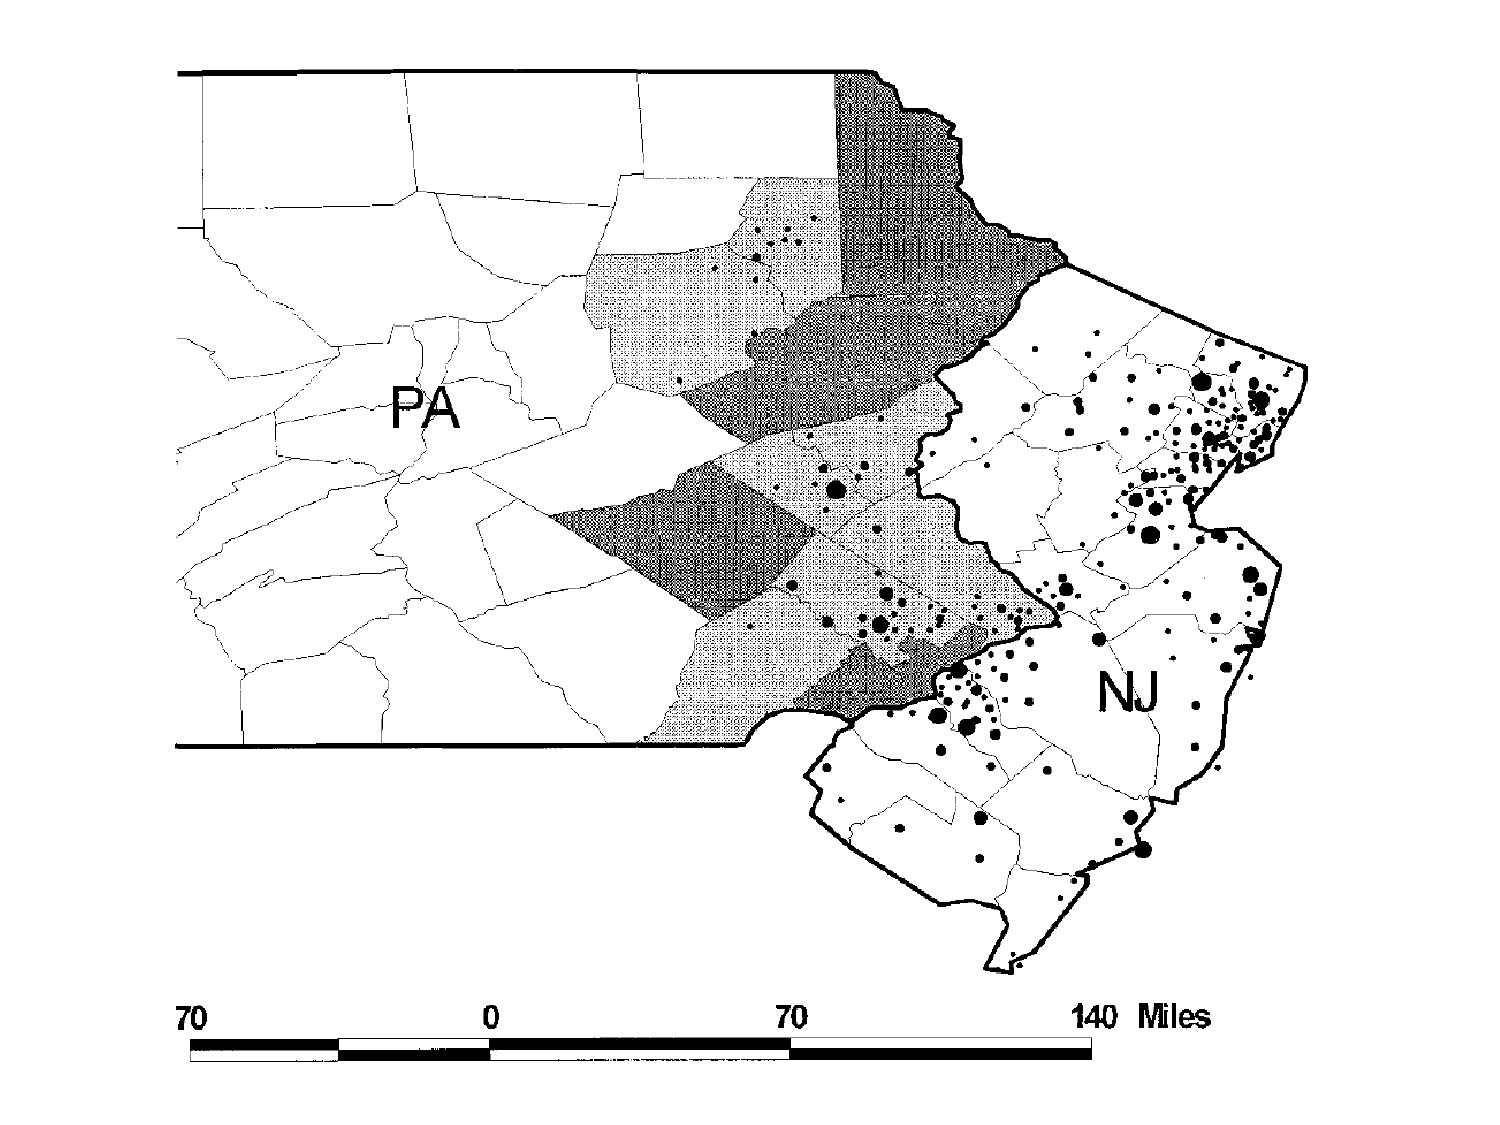
\includegraphics[height=3in,keepaspectratio=1]{CK1.pdf}
\end{center}
\end{frame}

\begin{frame}
  \frametitle{Sample Means: Minimum wage laws and employment}
\begin{center}
  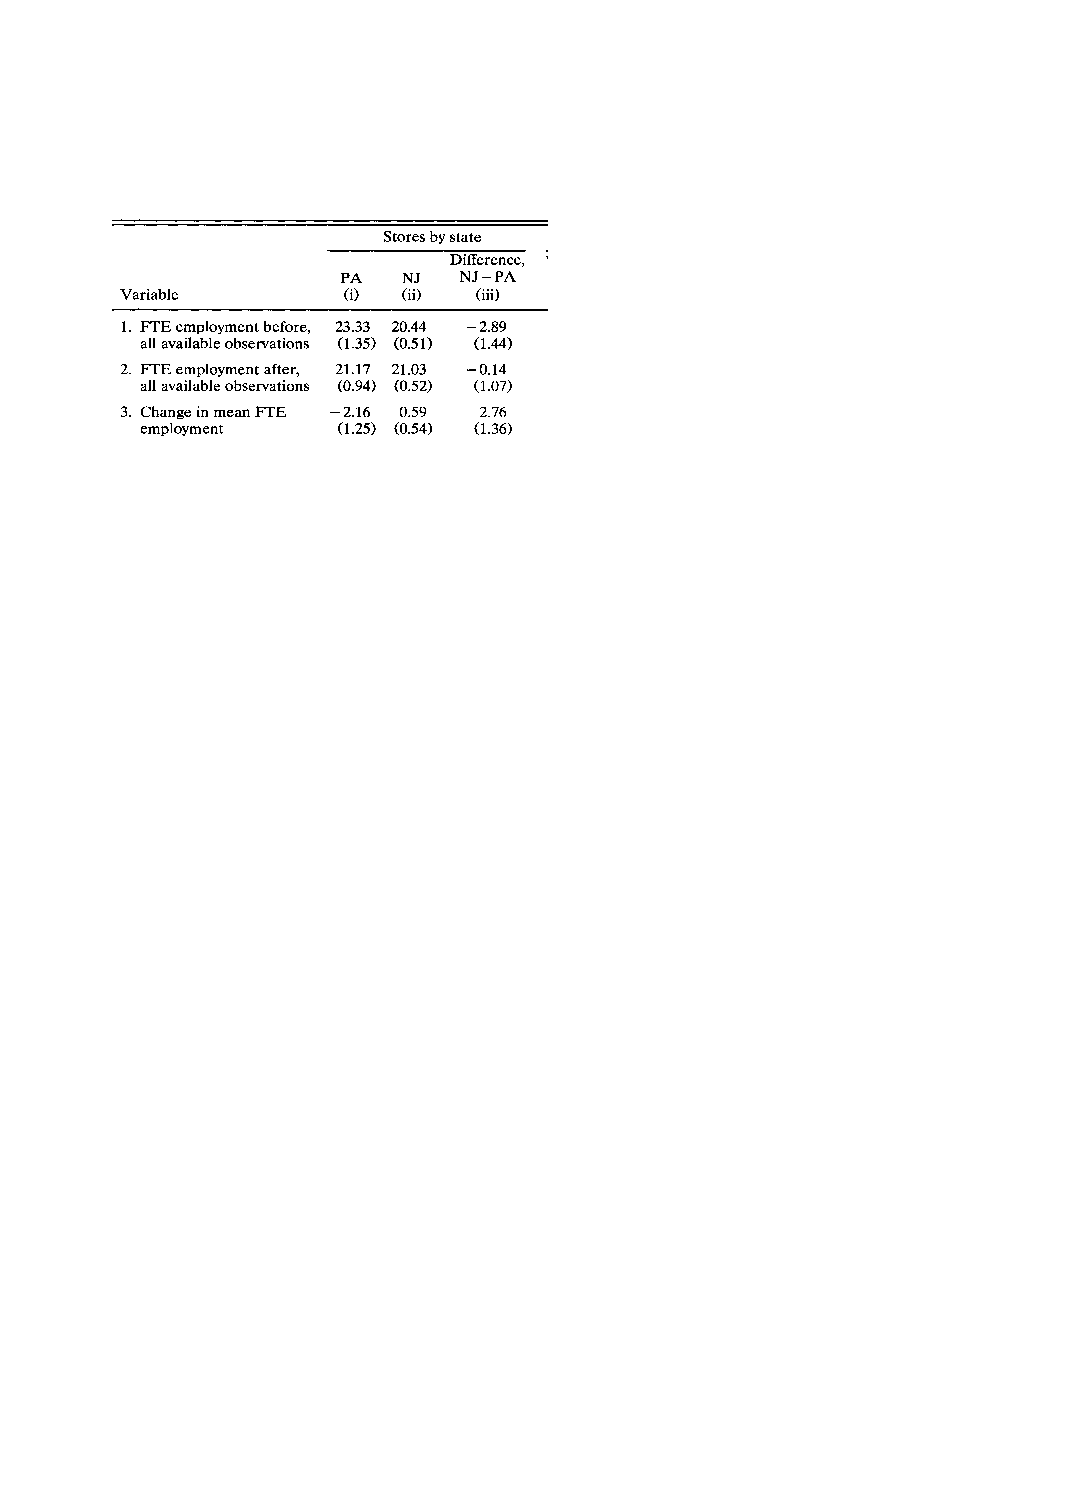
\includegraphics[height=2.4in,keepaspectratio=1]{CKresults1.pdf}
\end{center}
\end{frame}

%\begin{frame}
%  \frametitle{Difference-in-Differences: Estimators}
%\begin{esti}[Sample Means: Repeated Cross-Sections]\small
%Let
%$\{Y_i, D_i, T_i \}_{i=1}^n$ be the
%pooled sample (the two different cross-sections merged) where $T$
%is a random variable that indicates the period (0 or 1) in which the
%individual is observed.\\\bigskip The difference-in-differences estimator is given by:
%\begin{multline}
%\left\{\frac{\sum  D_i\cdot T_i\cdot Y_i}{\sum D_i\cdot T_i} -
%\frac{\sum  (1-D_i)\cdot T_i\cdot Y_i}{\sum (1-D_i)\cdot T_i}\right\}\\ -
%\left\{\frac{\sum D_i\cdot(1-T_i)\cdot Y_i}{\sum D_i\cdot(1-T_i)} -
%\frac{\sum (1-D_i)\cdot (1-T_i)\cdot Y_i}{\sum (1-D_i)\cdot (1-T_i)}\right\}\nonumber
%%\label{equation:sdid}
%\end{multline}
%\end{esti}
%\end{frame}

\begin{frame}
  \frametitle{Difference-in-Differences: Estimators}
\begin{esti}[Regression: Repeated Cross-Sections]\small
\textbf{In the two period case}, the same estimator can be computed by regression:
\[
Y = \mu + \gamma\cdot D + \delta\cdot T + \tau \cdot (D\cdot T) + \varepsilon,
\]
where $\E[\varepsilon|D,T]=0$.
\end{esti}\medskip
\onslide<2->
\begin{center}
\small
\begin{tabular}{c|c|c|c}

    {\bf } & {\bf After (T=1)} & {\bf Before (T=0)} & {\bf After - Before} \\
\hline \hline
\multirow{2}{*}{{\bf Treated D=1}}  & \multirow{2}{*}{$\mu + \gamma + \delta + \tau$} & \multirow{2}{*}{$\mu + \gamma$} & \multirow{2}{*}{$\delta + \tau$}    \\
 & & & \\
\hline
\multirow{2}{*}{{\bf Control D=0}}   & \multirow{2}{*}{$\mu +  \delta$} & \multirow{2}{*}{$\mu$} & \multirow{2}{*}{$\delta$}    \\
 & & & \\
\hline
\multirow{2}{*}{{\bf Treated - Control}}   & \multirow{2}{*}{$\gamma + \tau$} & \multirow{2}{*}{$\gamma$} & \multirow{2}{*}{$\tau$}    \\
 & & & \\
\hline
\end{tabular}
\end{center}
%Correct standard errors to account for temporal dependence!
\small
Again, parallel trends: ``time-effect'' $\delta$ same for treated and controls
\end{frame}

\begin{frame}[fragile]
  \frametitle{Regression: Minimum wage laws and employment}

\scriptsize
\begin{lstlisting}[language=R, basicstyle=\ttfamily]
> d <- read.dta("CK1994_longformat.dta",convert.factors = FALSE)
> head(d[, c('ID', 'nj', 'postperiod', 'emptot')])
  ID nj postperiod emptot
1  1  0          0  40.50
2  1  0          1  24.00
3  2  0          0  13.75
4  2  0          1  11.50
5  3  0          0   8.50
6  3  0          1  10.50
\end{lstlisting}
\end{frame}

% \begin{frame}[fragile]
%   \frametitle{Regression: Minimum wage laws and employment}

% \footnotesize
% \begin{lstlisting}[language=R, basicstyle=\ttfamily]
% with(d,
%  (
%   mean(emptot[nj == 1 & postperiod == 1], na.rm = TRUE) -
%   mean(emptot[nj == 1 & postperiod == 0], na.rm = TRUE)
%   )  -
%   (mean(emptot[nj == 0 & postperiod == 1], na.rm = TRUE) -
%   mean(emptot[nj == 0 & postperiod == 0], na.rm = TRUE)
%   )
%  )
% [1] 2.753606
% \end{lstlisting}
% \end{frame}


\begin{frame}[fragile]
  \frametitle{Regression: Minimum wage laws and employment}

You can reproduce the mean-differences estimator with a regression:
\footnotesize
\begin{verbatim}

> ols <- lm(emptot ~ postperiod * nj, data = d)
> coeftest(ols)

t test of coefficients:

              Estimate Std. Error t value Pr(>|t|)    
(Intercept)    23.3312     1.0719 21.7668  < 2e-16 ***
postperiod     -2.1656     1.5159 -1.4286  0.15351    
nj             -2.8918     1.1935 -2.4229  0.01562 *  
postperiod:nj   2.7536     1.6884  1.6309  0.10331
\end{verbatim}
%Note: Should adjust standard errors to account for temporal dependence
\end{frame}


\begin{frame}{Three famous DiD studies: is parallel trends credible?}
\footnotesize
For each: imagine a \textit{time-varying} confounder. What might make $\Delta Y(0)$ differ between treated and control?
\medskip
\begin{enumerate}
\item<1-> \textbf{Card \& Krueger (1994)}: NJ raises its minimum wage; PA doesn't.\\
  $Y$ = fast-food employment. Compare NJ vs PA, before/after.
\medskip
\item<2-> \textbf{Ashenfelter (1978)}: federal job-training program (MDTA/CETA). Trainees enroll; non-enrollees serve as controls.\\
  $Y$ = earnings. Compare trainees vs non-trainees, before vs after enrollment.
\medskip
\item<3-> \textbf{Autor (2003)}: US state courts recognized exceptions to the ``employment-at-will'' doctrine (make workers harder to fire) in different years. You look at whether there is more reliance on temporary workers (easier to fire). 
\medskip
\item<4-> Snow's cholera study: Lambeth (moves water works) vs. S\&V (does not move water works), look at cholera mortality. 
\end{enumerate}
\end{frame}

%\begin{frame}
%  \frametitle{DID with Covariates}
%\small
%\onslide<1-> Suppose you only believe parallel trends conditionally on covariates/ want to remove effect of change in some observables \\
%\smallskip
%\onslide<2->
%\begin{esti}[Regression: Repeated Cross-Sections]\small
%DID regression estimator with covariates:
%\[
%Y = \mu + \gamma\cdot D + \delta\cdot T + \tau \cdot (D\cdot T) + X^{\top}\beta + \varepsilon.
%\]\vspace*{-0.5cm}
%\begin{itemize}
%\item introducing time-invariant   $X$'s is not helpful (they get differenced-out)
%\item be careful with time-varying $X$'s: they may be  affected by the treatment
%%\item correct standard errors to account for temporal dependence
%\end{itemize}
%\textit{Can} interact time-invariant
%covariates with the time indicator:
%\begin{equation}
%Y = \mu + \gamma\cdot D + \delta\cdot T + \alpha\cdot (D\cdot T) + X^{\top}\beta_0 + (T\cdot X^{\top})\beta_1   +\varepsilon \nonumber
%%\label{equation:tvdid}
%\end{equation}
%... but typically strains credibility.
%\end{esti}
%\end{frame}

%\begin{frame}
%  \frametitle{Panel Version}
%\small
%  \onslide<1-> With panel data you have same units in pre- and post 
%  \begin{itemize}
%  \item efficiency gains possible: unit and period fixed effects 
%  \item still relying on parallel trends or ``no unobserved time-varying confounders''
%  \end{itemize}
%  \smallskip
%  
%\begin{esti}[Regression: Panel Data]\small
%\[
%Y_{it} = \mu + \gamma_i + \delta T + \tau D_{it} + X_{it}^{\top}\beta + \varepsilon_{it}
%\]\vspace*{-0.5cm}
%\footnotesize
%\begin{itemize}
%\item One intercept for each unit, $\gamma_i$
%\item $D_{it}$ now coded as 1 for treated in post-period and 0 otherwise ($D_i\cdot T_i$ from before)
%%\item Correct standard errors to account for temporal dependence
%\end{itemize}
%\small
%Equivalently, post-minus-pre difference then simple regression:
%\[
%\Delta Y_i = \delta + \tau \cdot D_i + \Delta X_i^{\top} \beta_{\Delta} + u_i,
%\]
%\footnotesize
%where $\Delta Y_i = Y_i(1)-Y_i(0)$, $\Delta X_i = X_{i1}-X_{i0}$, $u_i=\Delta \varepsilon_i$; $D_i=1$ for unit(s) that get treated.\\\bigskip
%%\begin{itemize}
%%\item Often helps with temporal dependence.
%%\item With two periods this gives the same result as other regressions
%%\end{itemize}
%%$\Rightarrow$ Can also add $X$ to explain differences in trends.
%\end{esti}
%\end{frame}
%
%\begin{frame}{Some Notes on Panel DID}
%\small
%\begin{itemize}
%\item<1-> With two periods, this panel FE approach is numerically equal to computing DID by hand or using first-differencing.\\
%\bigskip
%\begin{itemize}
%\item<2-> in this limited setting, the ``no time-varying confounders'' assumption we think of with regression is the same as the ``parallel trends'' assumptions. 
%\end{itemize}
%\bigskip
%\item<3-> This led to a craze in calling two-way FE estimators ``DID'' and calling the ``no time-varying confounders'' assumptiong ``parallel trends'' even in more complicated models with more than two periods and with staggered adoption. But things break down in those settings:
%
%\begin{itemize}
%\item using FEs doesn't always give you back an obvious DID estimator
%\item if you can sustain the conditional ignorability assumption/ no timer varying confounders, you are always fine, but there are subtle threats to this posed by issues such as effect of past $Y$ on future $Y$.
%\item many recent papers on this; we can discuss more if people want.
%\end{itemize}
%%\bigskip
%%\item<4-> Adding pre-treatment covariates to first-diff regression equivalent to adding them interacting with $T$ in the panel version.
%\end{itemize}
%\end{frame}

%\begin{frame}[fragile]
%  \frametitle{Regression: Minimum wage laws and employment}
%\onslide<1-> You can setup regression with unit and time FE by hand, or use PLM:
%\footnotesize
%\begin{verbatim}
%library(plm)
%library(lmtest)
%> d$Dit=d$nj * d$postperiod #Dit=1 only in post-tx
%> d=plm.data(d, indexes = c("ID", "postperiod"))
%> did.reg=plm(emptot~postperiod+Dit, data = d,model = "within")
%
%> coeftest(did.reg, vcov=function(x) 
%                 vcovHC(x, cluster="group", type="HC1"))
%t test of coefficients:
%            Estimate Std. Error t value Pr(>|t|)  
%postperiod1  -2.2833     1.2465 -1.8319  0.06775 .
%Dit           2.7500     1.3359  2.0585  0.04022 *
%\end{verbatim}
%\end{frame}
%
%\begin{frame}[fragile]
%
%  \frametitle{Regression: Minimum wage laws and employment}
%\onslide<1-> You can do first-differencing by hand then regress, or ask PLM:
%
%  \footnotesize
%\begin{verbatim}
%> firstdiff.mod=plm(emptot~postperiod*nj, data = d, model = "fd")
%
%>coeftest(firstdiff.mod, vcov=function(x) vcovHC(x, type="HC0"))
%
%t test of coefficients:
%
%               Estimate Std. Error t value Pr(>|t|)  
%postperiod1     -2.2833     1.2465 -1.8319  0.06775 .
%postperiod1:nj   2.7500     1.3359  2.0585  0.04022 *
%---
%\end{verbatim}
%\end{frame}

%\section{Difference-in-Differences: Threats to Validity}
%
%\begin{frame}
%  \frametitle{Difference-in-Differences: Threats to Validity}
%\small
%\begin{enumerate}
%\item Non-parallel trends \footnotesize(aka unequal time-effects, unobserved time-varying confounding) \medskip
%\small
%\item Compositional differences\medskip
%\item Long-term effects versus reliability\medskip
%\item Functional form dependence\medskip
%\end{enumerate}
%
%\onslide<2->  Bias is a matter of degree:
%\begin{itemize}
%\item small violations, small bias $\Rightarrow$ may be okay 
%\item but biases can be large, even give wrong sign
%\end{itemize}
%\bigskip
%
%\onslide<3-> With DID, the parallel trends assumption is often tough to sell, so be cautious
%\end{frame}


%\subsection{Non-parallel dynamics}

\begin{frame}{Some sneaky ways parallel trends can be violated}
\small
\begin{enumerate}
\footnotesize
\item<1-> \textbf{Ashenfelter dip / mean reversion}: treatment is a response to a recent bad draw (people enroll in a training program \textit{because} earnings just dipped; NGOs target villages that had a setback). The treated group is poised to recover even without treatment---so $\Delta Y(0)$ differs.
\medskip
\item<2-> \textbf{Compositional change}: with repeated cross-sections, the treated and control samples aren't the same units over time. If treatment triggers migration or selective exit, the sampled pool shifts across periods and observed $\Delta Y$ no longer estimates $\Delta Y(0)$.
\medskip
\item<3-> \textbf{Short window vs long-run relevance}: parallel trends is much more plausible over short horizons. Over long ones, too much else happens---and short-term effects generally don't extrapolate to long-term ones.
\medskip
\item<4-> \textbf{Functional-form dependence}: differencing is not scale-invariant. If outcomes grow at rates that depend on their \textit{levels}, trends won't be parallel even with purely static confounding. Parallel in levels $\neq$ parallel in logs.
\end{enumerate}

% \begin{itemize}
% \item Falsification Test: Under the parallel trends assumption during the periods $t=-1,0,1$, we have:
%       \[
%        E[Y(0)-Y(-1)|D=1]- E[Y(0)-Y(-1)|D=0]=0
%       \]
%       \item That is, apply DID estimator to $t=-1,0$ and test if $\alpha=0$
%   %    \item Can use similar placebo test with second control group or other placebo outcomes that
%  %     are known to be unaffected
% \end{itemize}
%\item \emph{Long-term effects vs. reliability}:
%\begin{itemize}
%  \item Parallel trends assumption for DD is more likely to hold over
%a shorter time-window. In the long-run, many other things may happen and confound the effect of the treatment.
%\item Should be cautious to extrapolate short-term effects to long-term effects
%\end{itemize}
\end{frame}

%\begin{frame}
%  \frametitle{Checks for Difference-in-Differences Design}
%\begin{enumerate}
% \item Falsification test using data for prior periods
% \begin{itemize}
%\item Given parallel trends during periods $t=-1,0,1$, we have:
%       \[
%        E[Y(0)-Y(-1)|D=1]- E[Y(0)-Y(-1)|D=0]=0
%       \]
%\item run placebo DD on data from $t=-1,0$ and test if $\alpha=0$. If not, your
%       estimate comparing $t=0$ and $t=1$ may be biased
% \end{itemize}\medskip \pause
%\item Falsification test using data for alternative control group
% \begin{itemize}
%\item if the placebo DD with the alternative control is different from the DD with the original control, then the original DD may be biased
% \end{itemize}\medskip \pause
%\item Falsification test using alternative placebo outcome that is not supposed to be affected by the treatment
% \begin{itemize}
% \item if DD from placebo outcome is non-zero, then the DD estimate for original outcome may be biased
%  \end{itemize}
%\end{enumerate}
%\end{frame}

\begin{frame}
  \frametitle{Checks for Difference-in-Differences Design}

\begin{center}
 Is the parallel-trends assumption testable?
 \end{center}
 \end{frame}
  
  \begin{frame} \frametitle{Checks for Difference-in-Differences Design}
  Two kinds of \textcolor{Red}{falsification} tests for non-parallel trends 
\bigskip
\begin{enumerate}
 \item<1-> Falsification test using data for prior periods 
 \begin{itemize}
\item Given parallel trends during periods $t=-1,0,1$, we have:
       \[
        \E[Y_0-Y_{-1}|D=1]- \E[Y_0-Y_{-1}|D=0]=0
       \]
\item run placebo DID on data from $t=-1,0$. 
\item what ``treatment effect'' should we get?
\end{itemize}\medskip
%\item<2-> Falsification test comparing control groups
%%\begin{itemize}
%%\item if the placebo DID with the alternative control is different from the DID with the original control, then the original DID may be biased
%%\end{itemize}\medskip
\item<2-> Falsification test using alternative outcome or treated sub-group that is not supposed to be affected by the treatment
\begin{itemize}
\small
\item troubling if DID from the placebo outcome or un-movable group is non-zero.  \end{itemize}
\end{enumerate}
\end{frame}

\begin{frame}
  \frametitle{Falsification test: Data for prior periods}
  \vspace{-.2in}
\begin{center}
  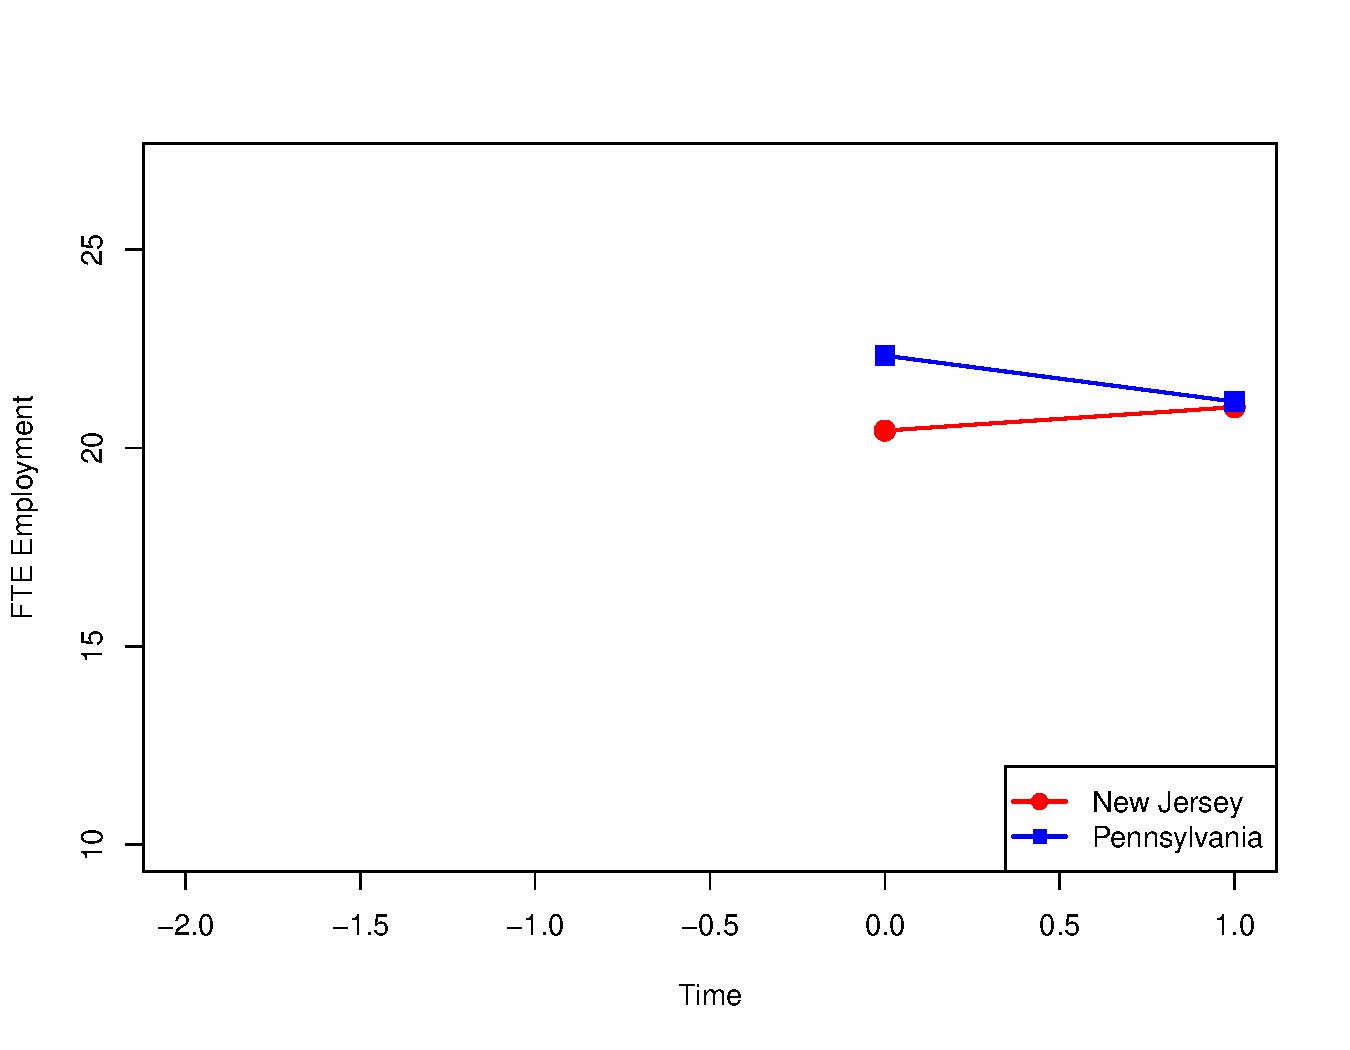
\includegraphics[scale=.4]{KCfalsification1.pdf}
\end{center}
\end{frame}


\begin{frame}
  \frametitle{Falsification test: Data for prior periods}
  \vspace{-.2in}
\begin{center}
  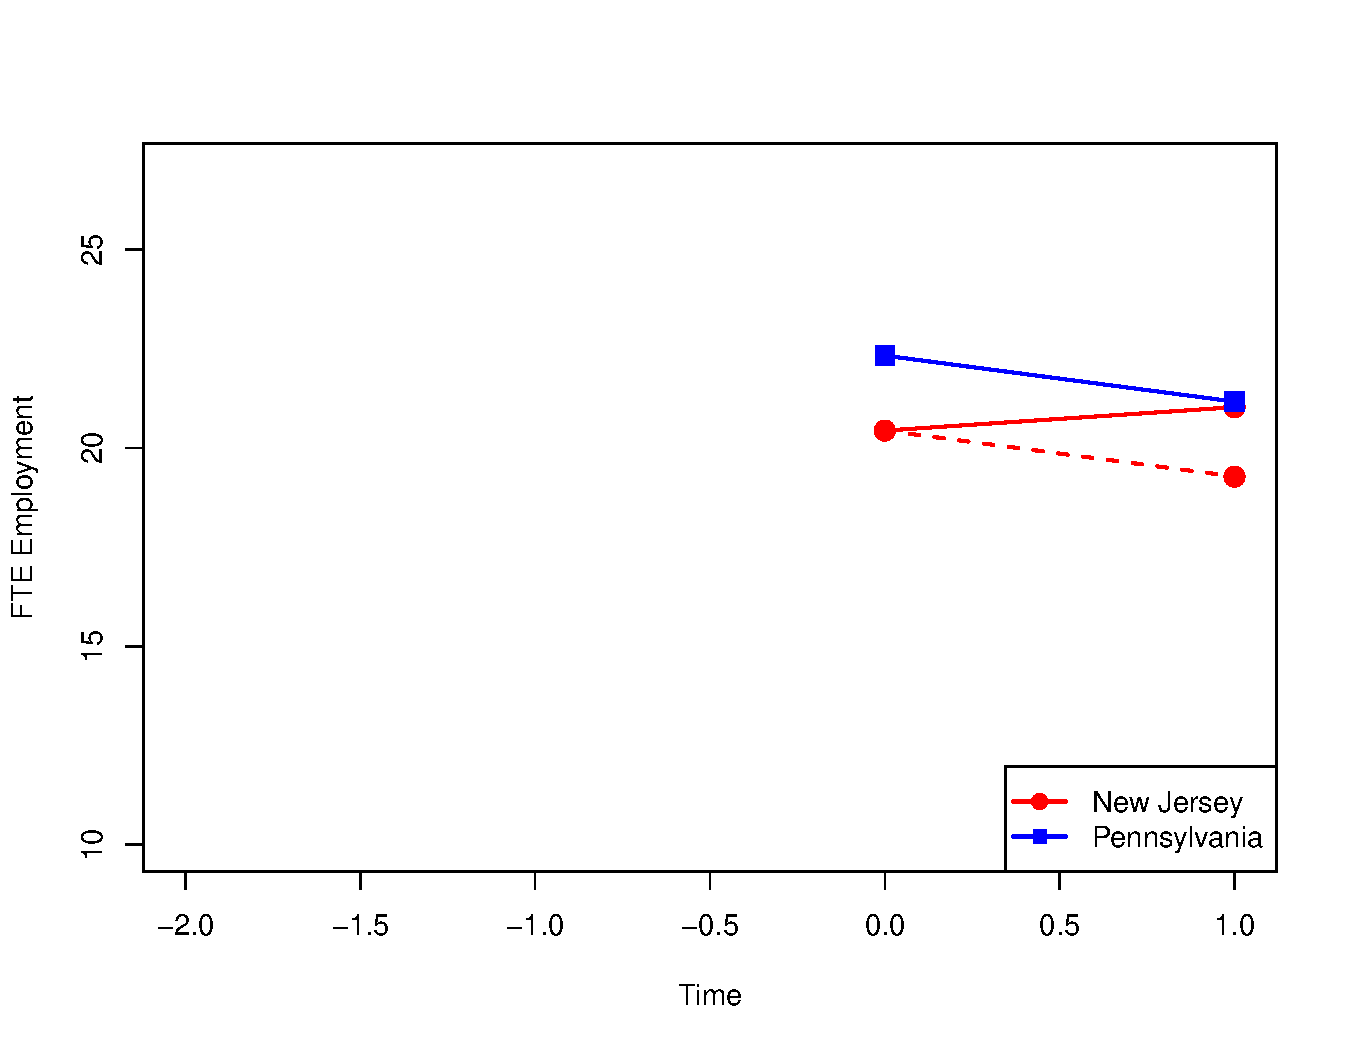
\includegraphics[scale=0.4]{KCfalsification2.pdf}
\end{center}
\end{frame}

\begin{frame}
  \frametitle{Falsification test: Data for prior periods}
  \vspace{-.2in}
\begin{center}
  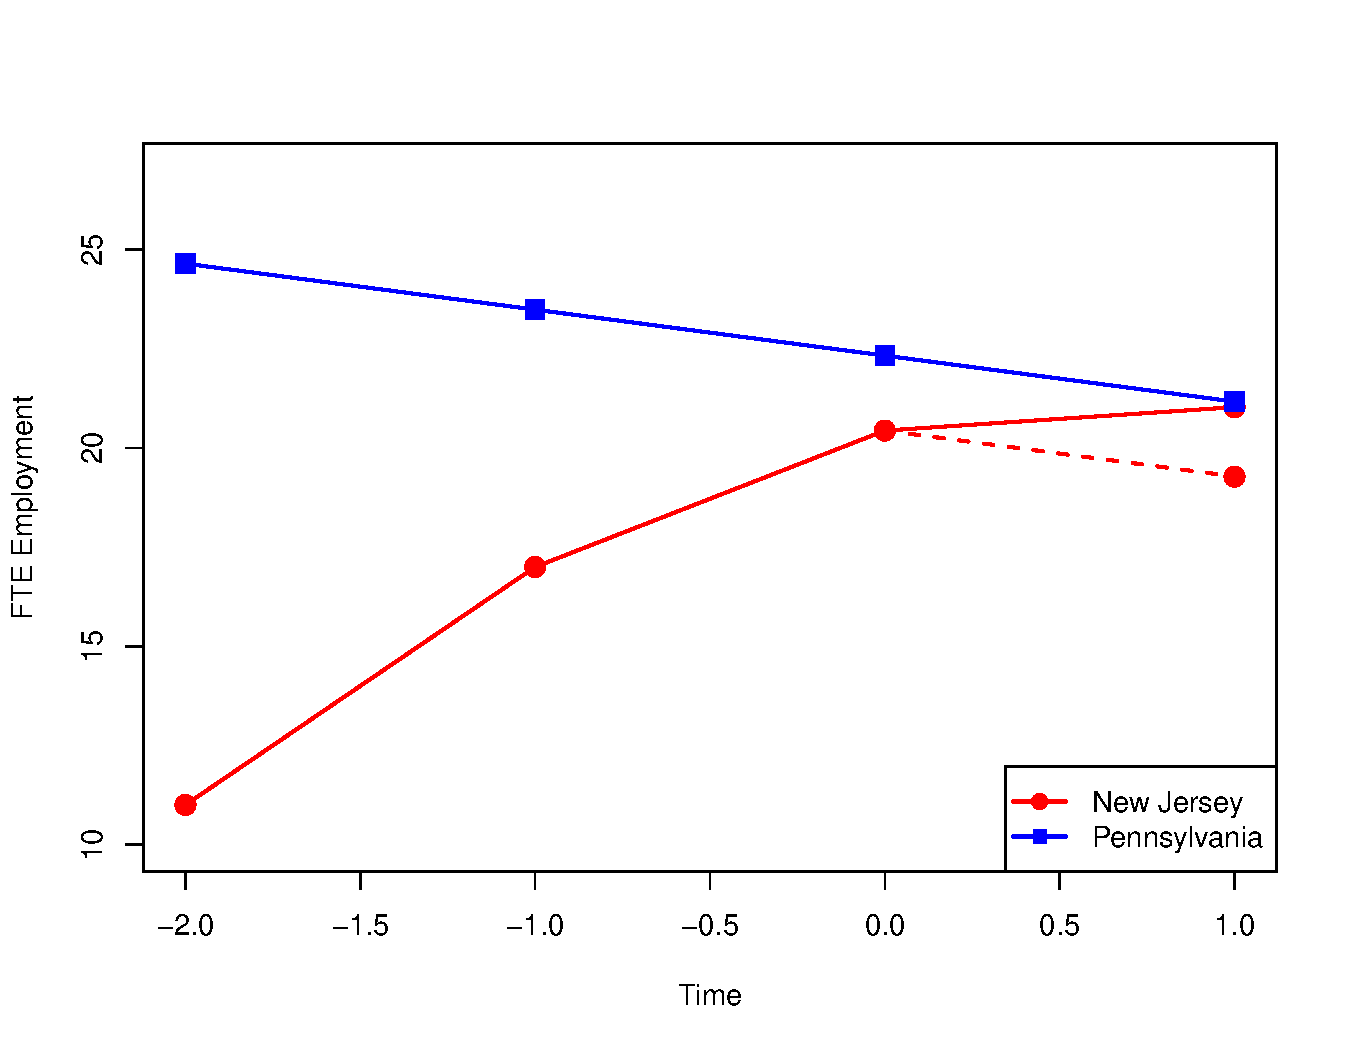
\includegraphics[scale=0.4]{KCfalsification4.pdf} \\
  Definitely bad.
\end{center}
\end{frame}


\begin{frame}
  \frametitle{Falsification test: Data for prior periods}
  \vspace{-.2in}
\begin{center}
  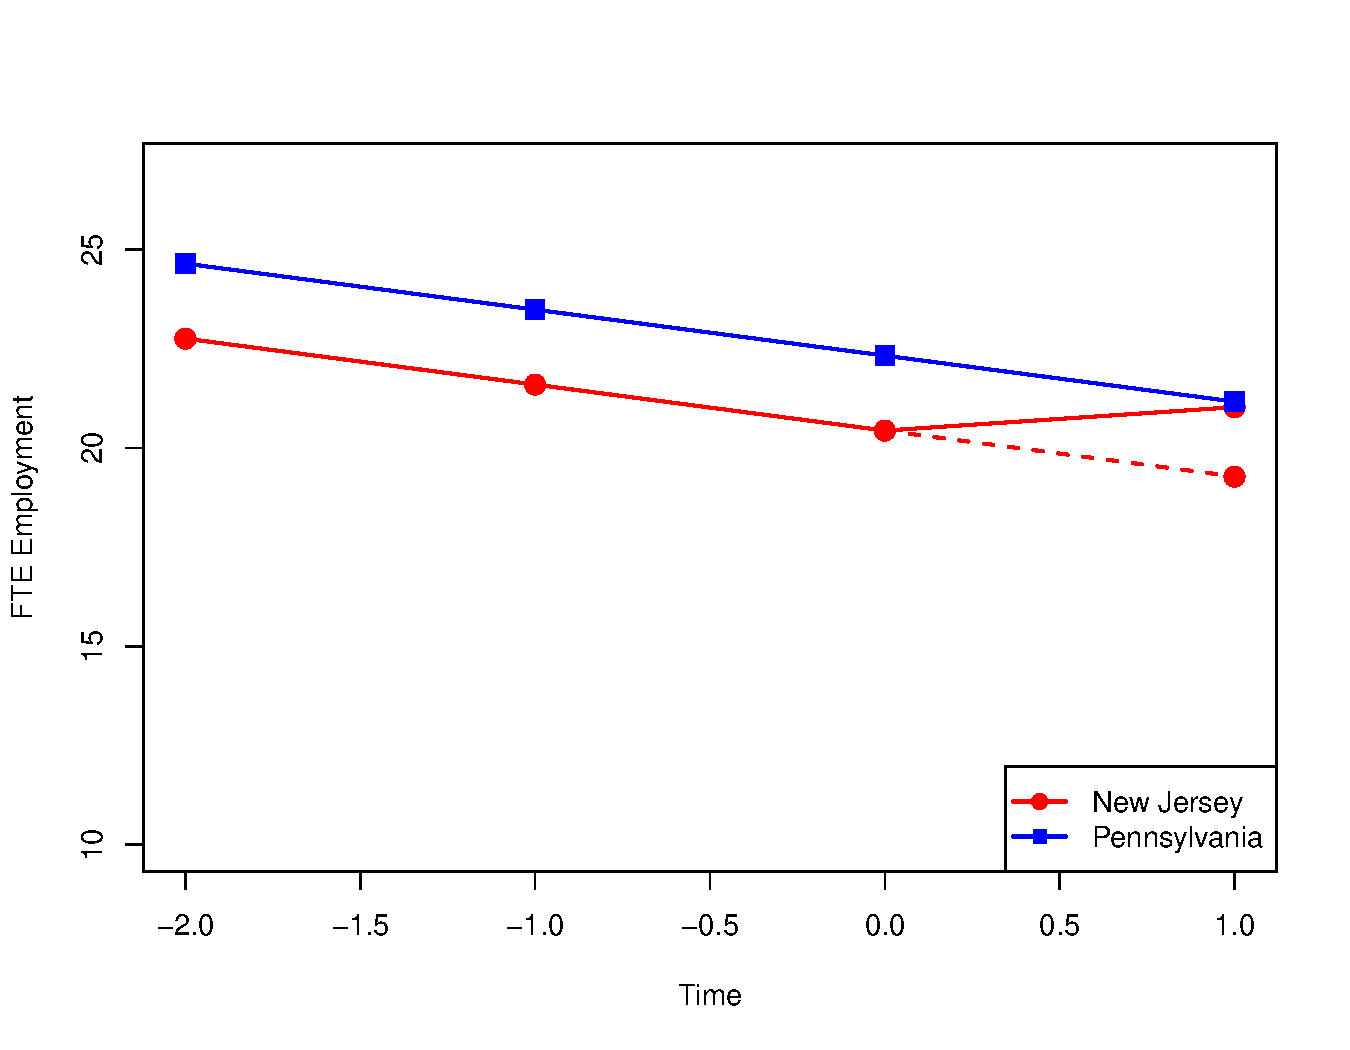
\includegraphics[scale=0.35]{KCfalsification3.pdf}\\
\onslide<2-> Not definitely bad, but why did they take treatment then? \\
\onslide<3-> Parallel pre-trends $\neq$ parallel trends. \\
\onslide<4-> You cannot test parallel trends.
\end{center}
\end{frame}



\begin{frame}{Other approaches to worrying about parallel trends}
\begin{enumerate}
\item \textbf{Sensitivity/ partial ID}\bigskip
\small
\begin{itemize}
\item Best-known is perhaps Rambachan \& Roth (2023)
\item Suggests checking if the effect estimate can survive non-parallelness $k$ times larger than the non-parallelness in the prior trends. 
\item A lot of papers don't even survive at $k=1$, which is clearly bad (Chiu, Lan, Liu, Xu, \textit{APSR} 2025)
\item Of course there is no (convincing) rule for ``how big of a $k$ is big enough''
\end{itemize}
\bigskip

\onslide<2-> We won't cover as much as I like but there are other ID opportunities for similar settings, and other sensitivity analyses depending on what you are prepared to reason about.\\
\medskip
\onslide<2-> Vote in the comments to affect the story.
\end{enumerate}
\end{frame}

%
%\begin{frame}
%  \frametitle{Longer Trends in Employment (Card \& Krueger 2000)}
%  \vspace{-.1in}
%\begin{center}
%  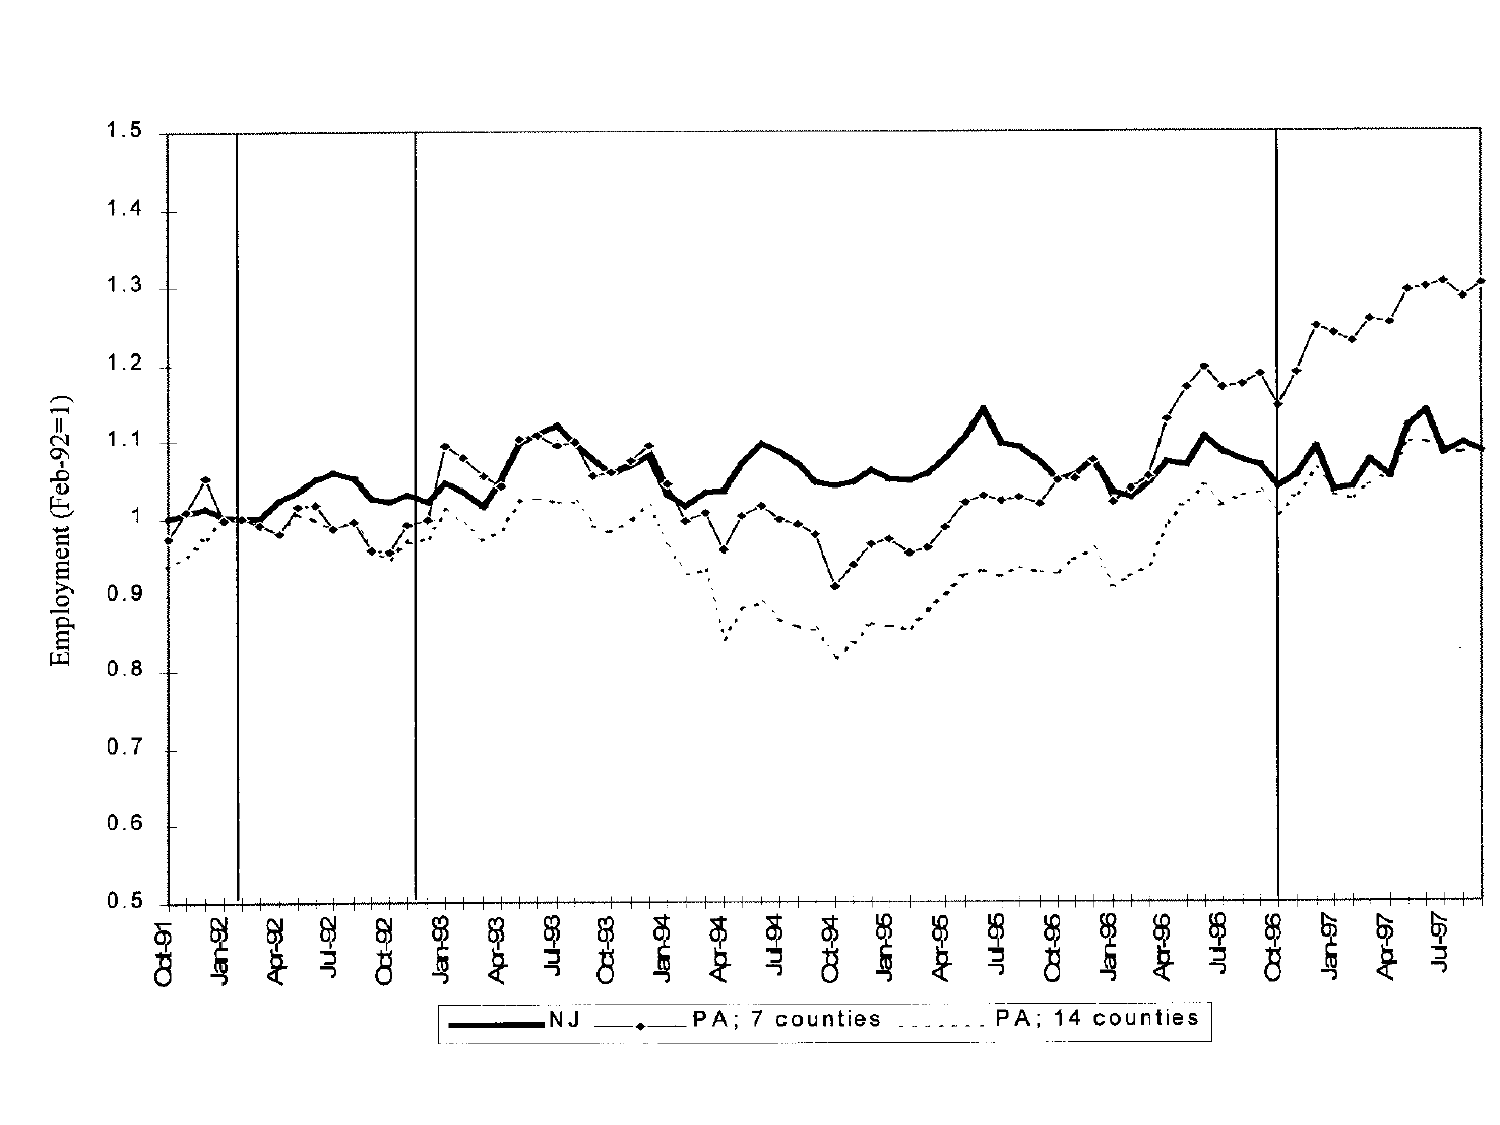
\includegraphics[height=3in,keepaspectratio=1]{PreTrend.pdf}
%\end{center}
%\end{frame}


%\begin{frame}
%  \frametitle{Falsification test: Compare control groups}
%  \vspace{-.2in}
%\begin{center}
%  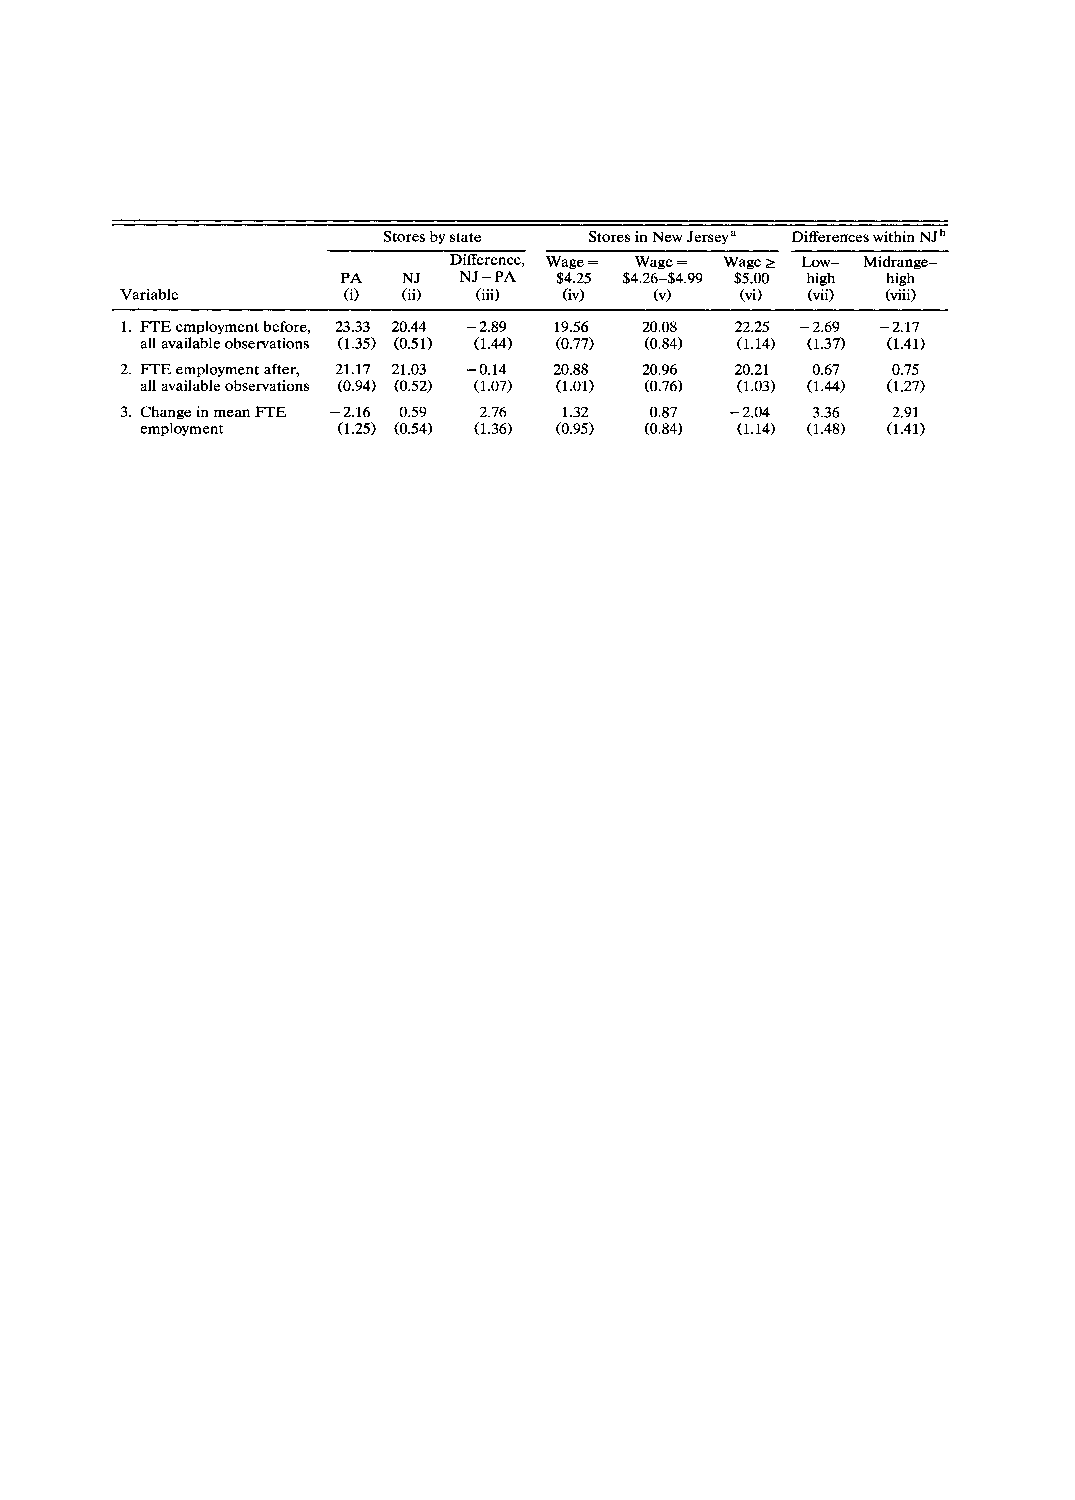
\includegraphics[height=1.3in,keepaspectratio=1]{CKresults4.pdf}
%\end{center}
%% \begin{itemize}
%%\item
%Both midrange and high wage stores in NJ are control groups, but have an apparent ``effect''
%%If placebo DID between original and alternative control group is not zero, then the original DID may be biased
%% \end{itemize}\medskip \pause
%\end{frame}


%
%\begin{frame}
%  \frametitle{Triple Diff: Mandated Maternity Benefits (Gruber, 1994)}
%\hspace*{0.5cm}\begin{overprint}
%\onslide<1|handout:1>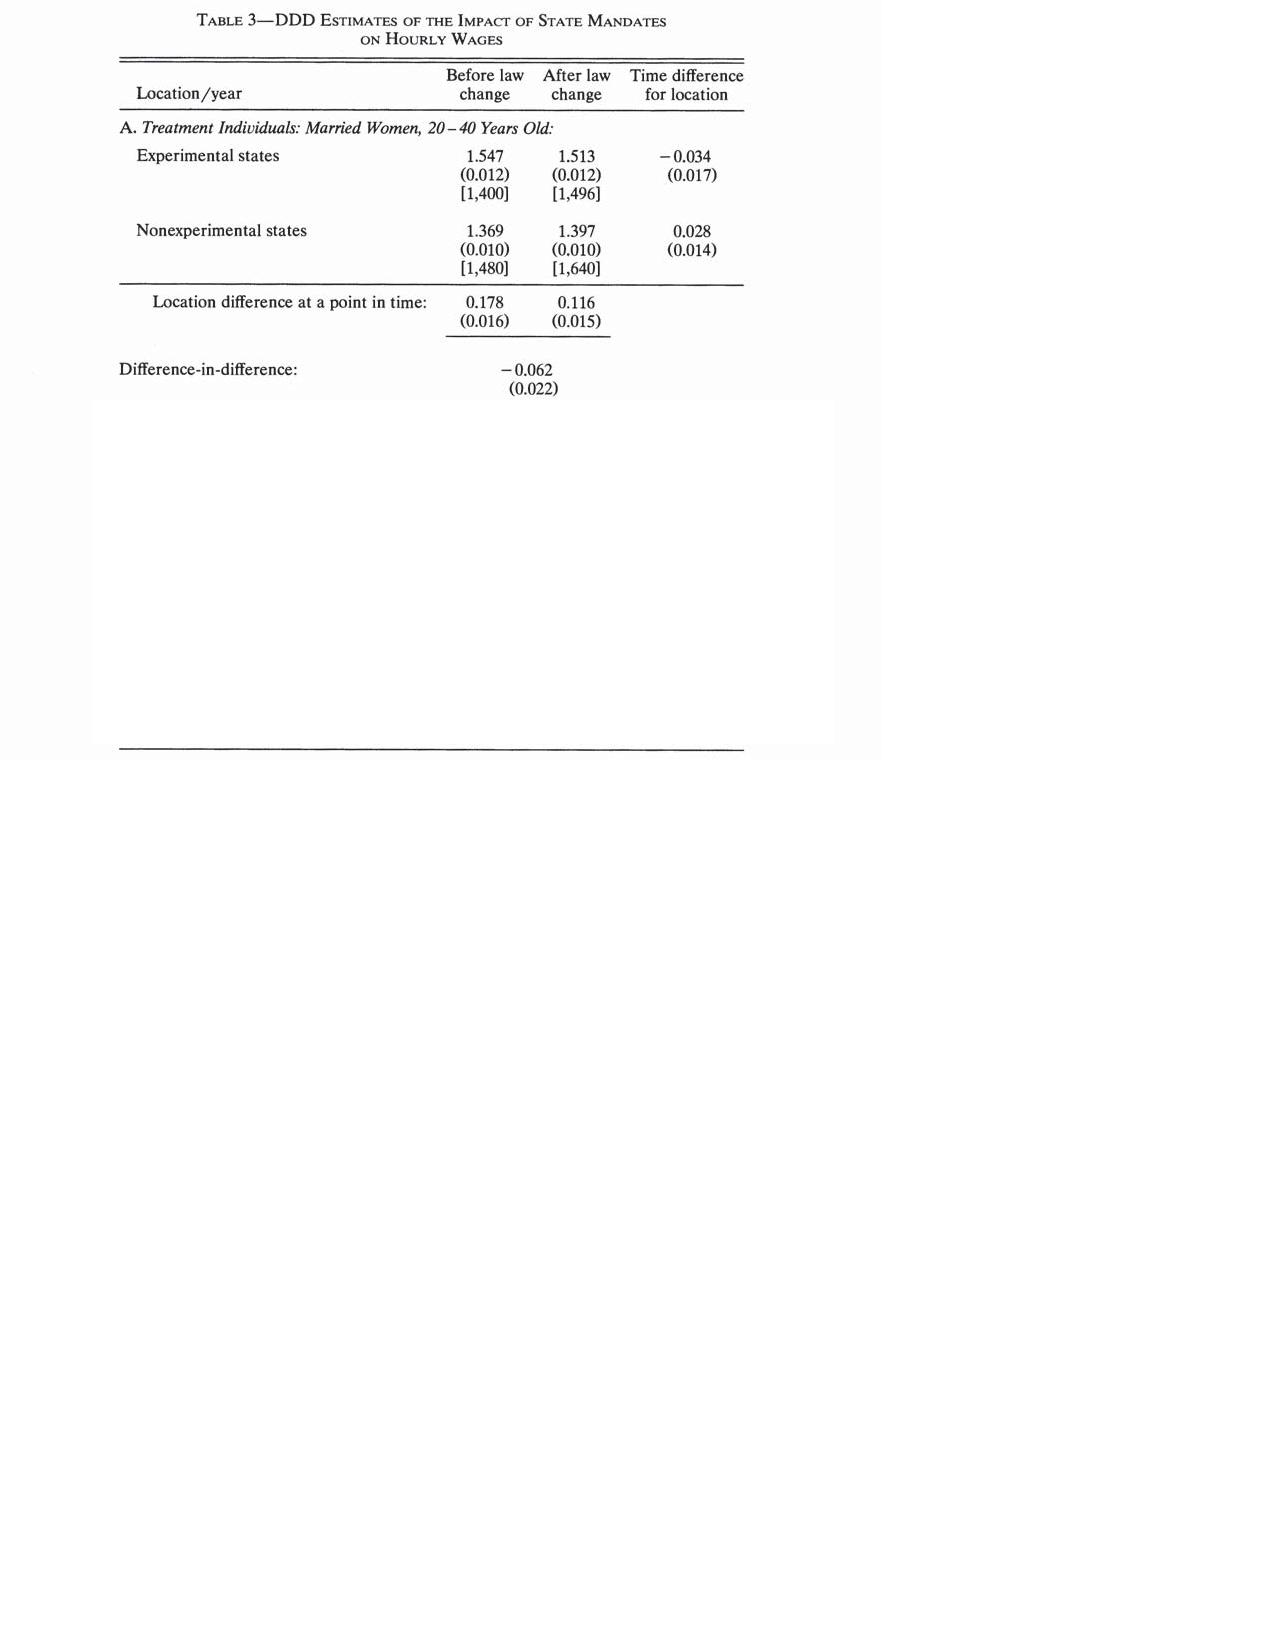
\includegraphics[height=3in,keepaspectratio=1]{DDD1markup.pdf}
%\onslide<2|handout:2>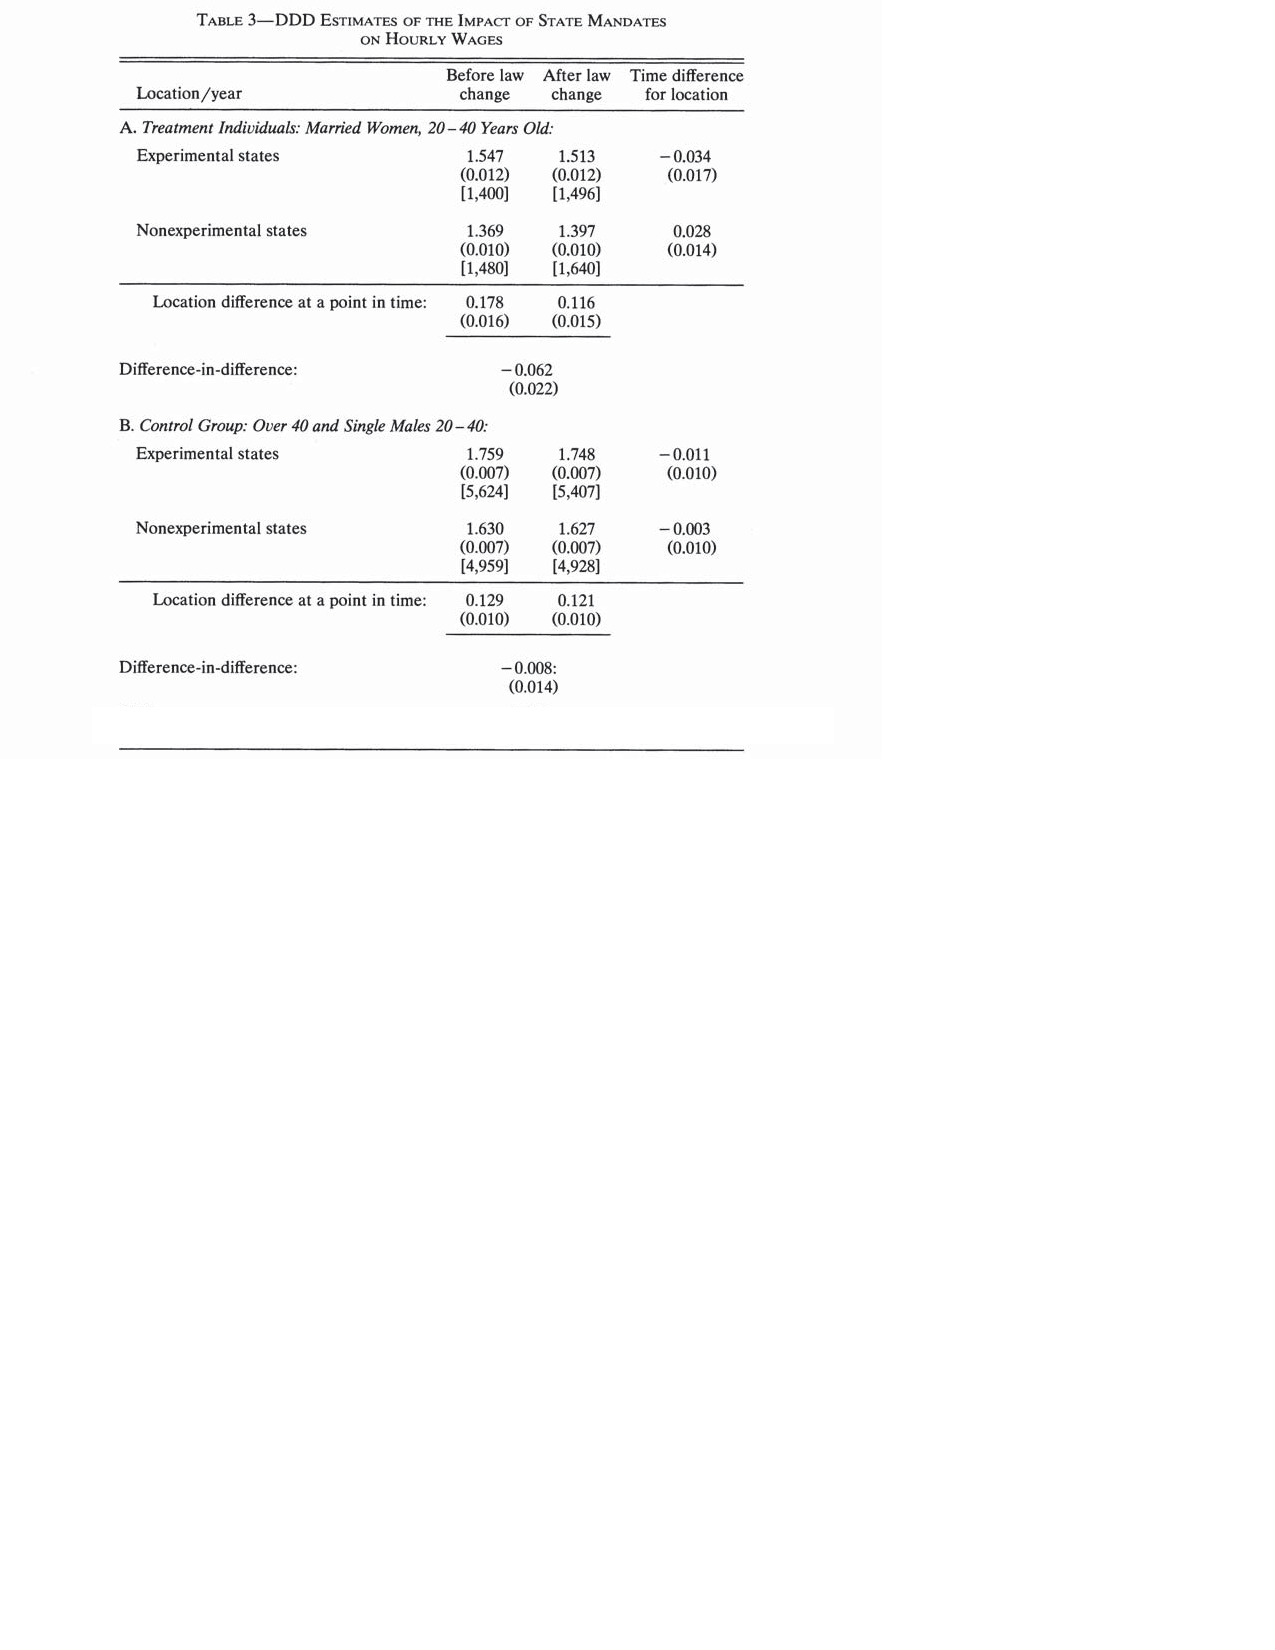
\includegraphics[height=3in,keepaspectratio=1]{DDD2markup.pdf}
%\onslide<3|handout:3>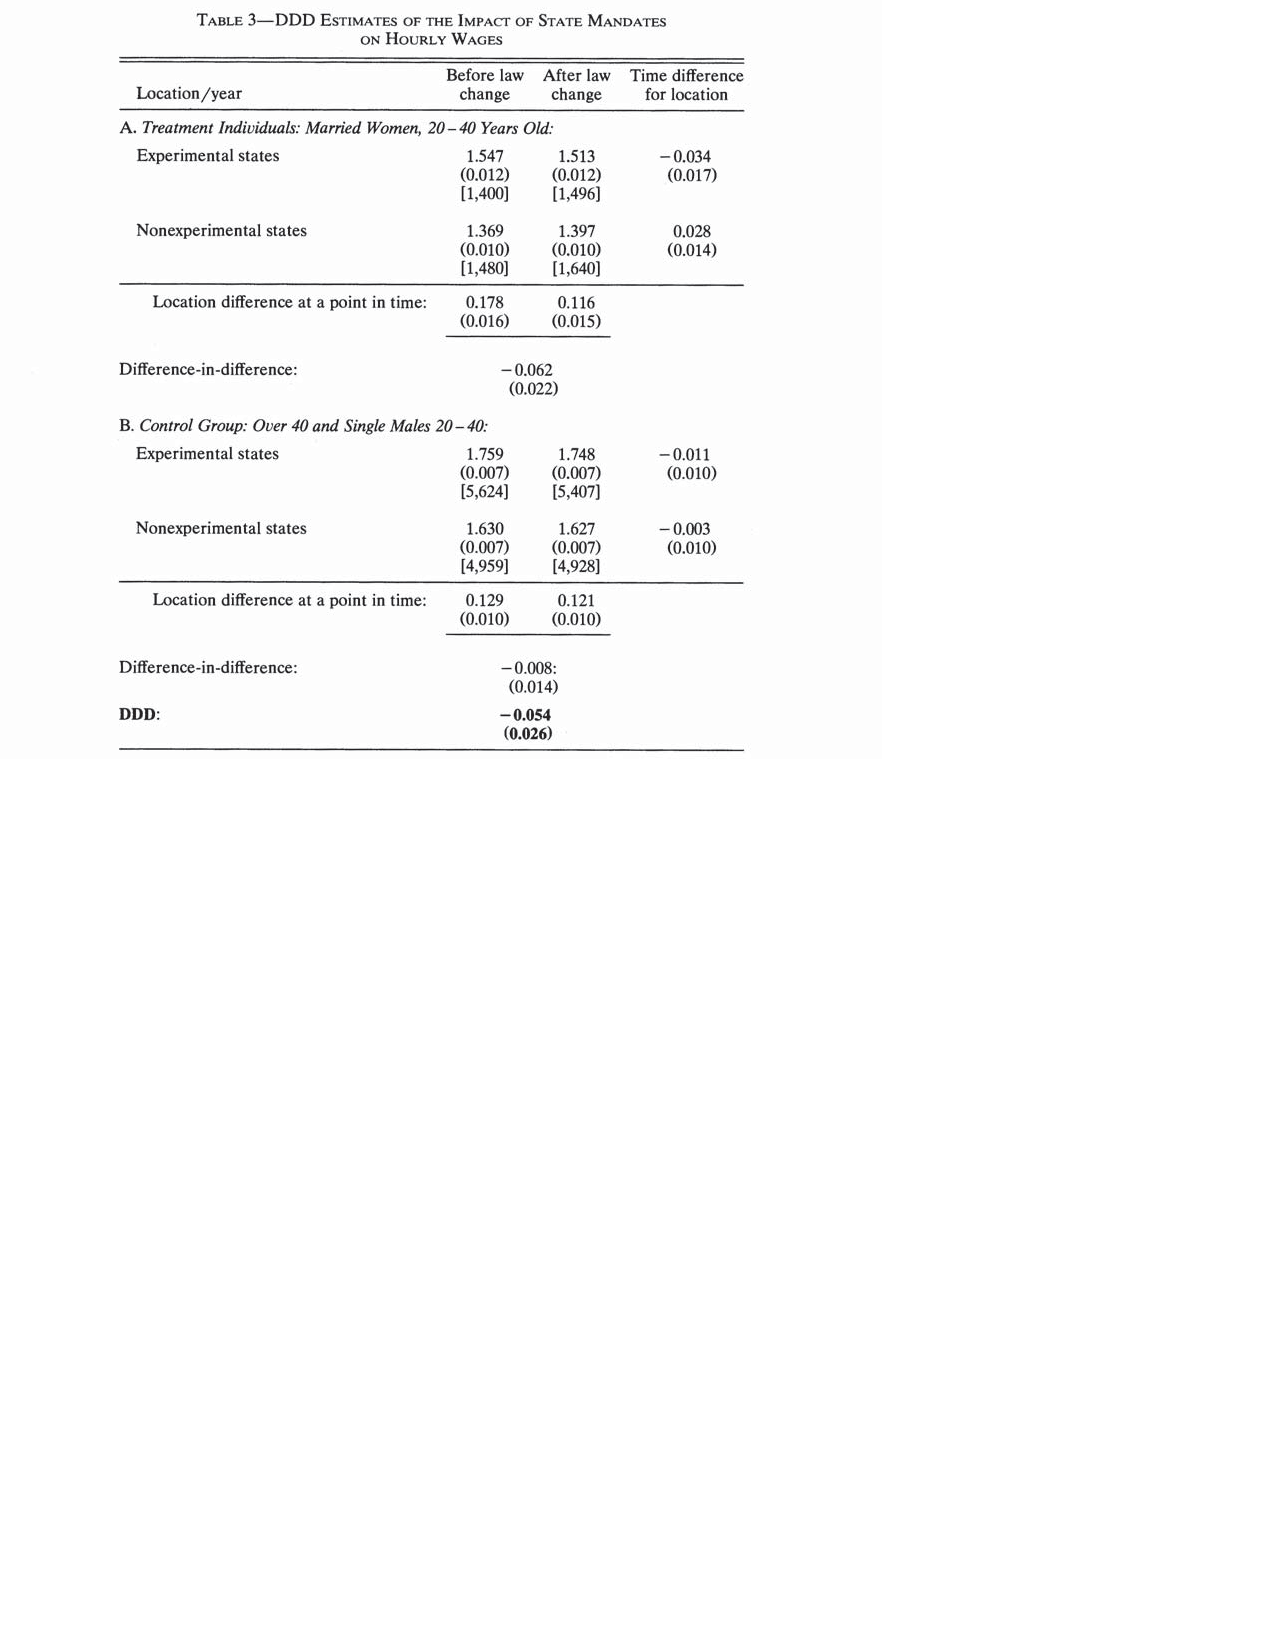
\includegraphics[height=3in,keepaspectratio=1]{DDDmarkup.pdf}
%\end{overprint}
%\end{frame}
%
%\begin{frame}
%  \frametitle{How useful is the Triple Diff/DDD?}
%  \onslide<1-> There could be compelling use cases, but... \\\
%\begin{itemize}
%  \item<2-> The DDD estimate is the difference between the DID of interest and the placebo DID (that is supposed to be zero)\bigskip
%  \begin{itemize}
%    \item<3-> If the placebo DID is non zero, it might be difficult to convince reviewers that the DDD removes all the bias\medskip
%    \item<4-> If the placebo DID is zero, then DID and DDD give the same results but DID is preferable because standard errors are smaller
%  \end{itemize}
%\end{itemize}
%\end{frame}
%
 

%\section{Example: Gerhard Schr\"oder's Flood}
%
%\begin{frame}
%  \frametitle{The Elbe Valley}
%  \vspace{-.06in}
%\begin{center}
%  \includegraphics[height=3.1in,keepaspectratio=1]{elbe1.pdf}
%\end{center}
%\end{frame}
%
%
%%\begin{frame}
%%  \frametitle{The Elbe Valley: 2001 and 2002}
%%  \vspace{-.06in}
%%\begin{center}
%%  \includegraphics[height=3.1in,keepaspectratio=1]{NASA.pdf}
%%\end{center}
%%\end{frame}
%
%\begin{frame}
%  \frametitle{Schr\"oder Sends the Troops}
%\begin{columns}
%  \begin{column}{0.5\textwidth}
%    \centerline{\includegraphics[height=1.2in,keepaspectratio=1]{flood1.pdf}}
%    \centerline{\includegraphics[height=1.2in,keepaspectratio=1]{flood2.pdf}}
%
%
%  \end{column}
%
%  \begin{column}{0.3\textwidth}
%    \centerline{\includegraphics[height=1.2in,keepaspectratio=1]{flood3.pdf}}
%    \centerline{\includegraphics[height=1.2in,keepaspectratio=1]{flood4.pdf}}
%  \end{column}
%\end{columns}
%
%\end{frame}
%
%%\begin{frame}
%%  \frametitle{Gerhard Schr\"oder's Flood}
%%
%%  \begin{itemize}
%%    \item Panel data for Germany's 299 electoral districts. $Y$: PR-vote share of Social Democratic Party SPD\bigskip
%%    \item Two periods
%%    \begin{itemize}
%%      \item $T=0$: Federal election 1998
%%      \item $T=1$: Federal election 2002
%%      \item The Elbe flood occurred in August of 2002 and the election was held in September of 2002
%%      \end{itemize}\bigskip
%%   \item Treatment: Flooded Districts
%%   \begin{itemize}
%%     \item $D=1$ Flooded districts (all of which received federal disaster aid)
%%     \item $D=0$ Unaffected districts
%%   \end{itemize}
%%  \end{itemize}
%%\end{frame}
%

%\subsection{Long-term effects versus reliability}


%
%\begin{frame}
%  \frametitle{Compositional differences?}
%  \vspace{-.4in}
%\begin{center}
%  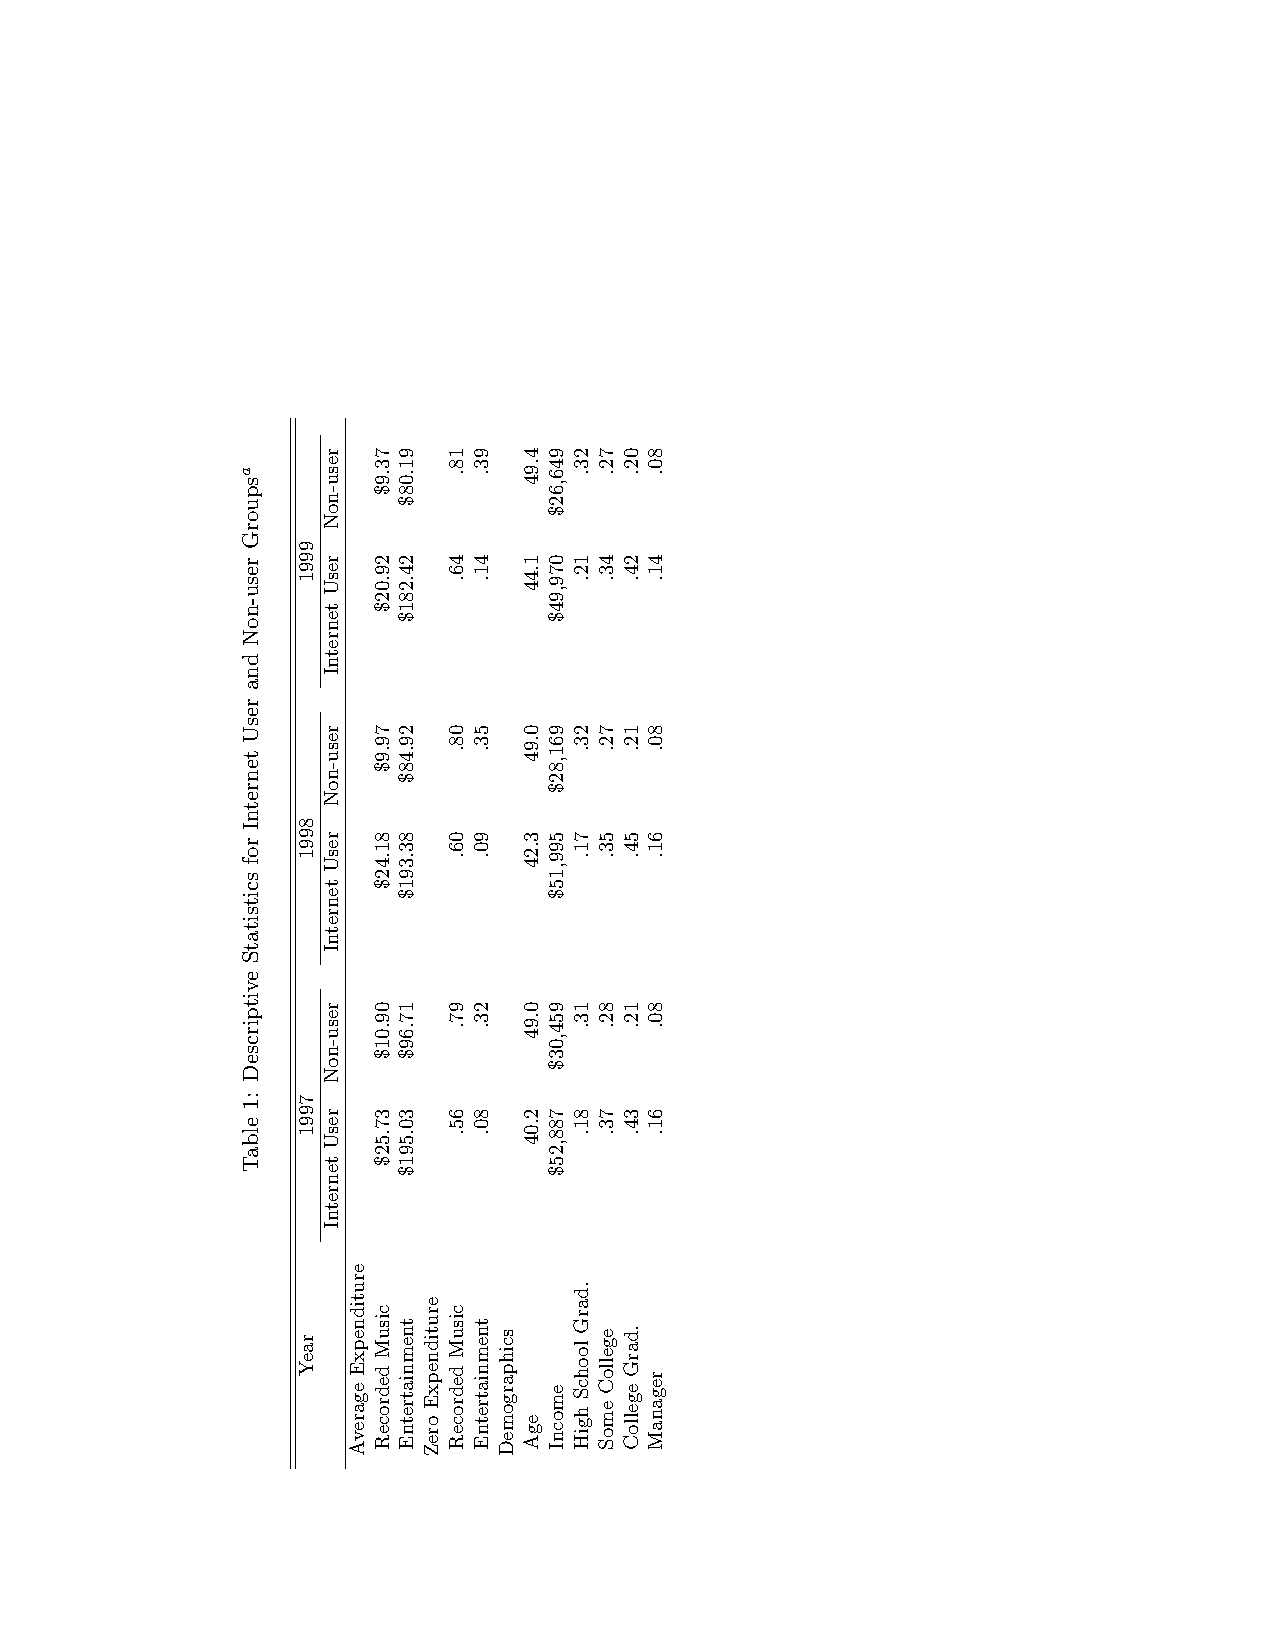
\includegraphics[height=4.6in,angle=270,keepaspectratio=1]{Jong20111.pdf}
%\end{center}  \vspace{-.0in}
%\onslide<2-> You can check for DID effect on the demographic outcomes as a test for compositional differences
%\end{frame}


%\begin{frame}
% \frametitle{Political Rewards for Flood Aid}
%  \vspace{-.2in}
% \begin{itemize}
%   \item Bechtel and Hainmueller (2011) consider relief spending in the context of the 2002 Elbe flooding in Germany, to estimate short- and long-term electoral returns to targeted policy benefits.
% \end{itemize}
%\begin{center}
%  \includegraphics[height=2.1in,keepaspectratio=1]{elbe1.pdf}
%  \includegraphics[height=2.2in,keepaspectratio=1]{flood4.pdf}
%\end{center}
%\end{frame}
%
%\begin{frame}
%  \frametitle{Political Rewards for Flood Aid}
%  \vspace{-.06in}
%\begin{center}
%  \includegraphics[height=2.8in,keepaspectratio=1]{elbe2.pdf}
%\end{center}
%\end{frame}
%
%\begin{frame}
%  \frametitle{Political Rewards for Flood Aid}
%  \vspace{-.06in}
%\begin{center}
%  \includegraphics[height=2.8in,keepaspectratio=1]{elbe3.pdf}
%\end{center}
%\end{frame}



%\section{Difference-in-Differences: Further Issues}

%\begin{frame}
%  \frametitle{Conditioning on Lagged Outcomes}
%
%\begin{itemize}
%\item Difference-in-Differences identification:
%\[
%\Delta Y_i = \delta + \tau{DD} \cdot D_i + u_i,
%\]
%where $\Delta Y_i = Y_i(1)-Y_i(0)$ and $u_i=\Delta \varepsilon_i$.
%\begin{itemize}
%  \item idea: remove bias from time-invariant unobservables
%\end{itemize} \bigskip
%
%\pause
%\item Alternative identification is to condition on pre-period outcome:
%\[
%Y_{i,t=1} = \beta_0 + \rho Y_{i,t=0} + \tau{SOO} \cdot D_{i} + \varepsilon_{i}
%\]\vspace{-.2in}  \pause
%\begin{itemize}
%  \item idea: once pre-period outcome is controlled for, selection on observables holds
%\end{itemize}
%\item Models are non-nested: Try both (with sufficient overlap on $Y_{i,t=0}$) \pause
%\end{itemize}
%\end{frame}
%
%\begin{frame}
%  \frametitle{Conditioning on Pre-Period Employment}
%  \vspace{-.2in}
%\begin{center}
%  \includegraphics[height=2.5in,keepaspectratio=1]{CKresults5.pdf}
%\end{center}
%\end{frame}

%\subsection{Functional form dependence}

\begin{frame}{``Modern'' DID?}
\small
\begin{itemize}
\item<1-> Classic DID above was two groups, two periods. Often you have units moving into treatment at different times (``staggered adoption''), and you'd still like to rely on something like parallel trends.
\item<2-> People long used ``two-way fixed effect'' regressions in these cases and unfortunately called this DID.
\item<3-> The trouble with TWFE is the combined result of:
\begin{itemize}
\footnotesize
\item<4-> \textbf{Already-treated units end up as ``controls''} for later cohorts' comparisons (mechanical; peculiar to staggered panels).
\item<5-> \textbf{Effect heterogeneity} across cohorts or time-since-treatment.
\end{itemize}
\item<6-> Intuition: with homogeneous effects, TWFE implicitly ``adjusts'' the already-treated controls back to their counterfactual by subtracting the one constant $\tau$. Under heterogeneity, no single adjustment works---so contaminated ``controls'' bleed into the estimate.
\end{itemize}
\end{frame}


\begin{frame}{Staggered DID: the core idea}
\small
\textbf{It is simple at bottom:}
\begin{itemize}
\item<1-> You could imagine a DID at each relevant time point estimating the \textbf{cohort-time effect} $ATT(g,t)$: the ATT at time $t$ for the cohort first treated at time $g$.\medskip
\item<2-> If these are well formed (choosing appropriate controls each time) then it's just a question of how to average up the $ATT(g,t)$'s.\medskip
\item<3-> Modern DID just points out that you need to construct these then \textit{explicitly} weight them.
\end{itemize}
\bigskip
\onslide<4-> Simplest fallback: run a clean 2$\times$2 DID for each adoption wave, look at them, average however you want.
\end{frame}


\begin{frame}{Estimators for Staggered DID}
\small
% \onslide<1-> See Chiu, Lan, Liu, Xu (\textit{APSR} 2025) for a great review of 6 estimators and their empirical impact, or the \texttt{fect} tutorial on 5 methods at \\
% \url{https://yiqingxu.org/packages/fect/05-panel.html}
% \par\bigskip
\onslide<1-> The main approaches are:
\scriptsize
\begin{tabular}{|p{2.8cm}|p{7.5cm}|}
\hline
\textbf{Approach} & \textbf{What it does} \\
\hline
Sun \& Abraham (2021) & Event-study estimator using cohort-specific relative-time indicators; avoids contamination from already-treated units; valid under heterogeneous effects and staggered timing. \\
\hline
Callaway \& Sant'Anna (2021) & Estimates group-time $ATT(g,t)$ using only not-yet-treated units as controls; flexible aggregation; avoids negative weighting. \\
\hline
Borusyak, Jaravel \& Spiess (2021); Liu, Wang \& Xu (2022) & Fits $Y(0)$ model with unit $+$ time FEs on \textit{untreated cells only}, impute $\hat Y_{it}(0)$ for treated cells, then aggregate effect estimates explicitly. Essentially g-computation with FE predictors. Implemented in \texttt{fect}. \\
\hline
de Chaisemartin \& D'Haultfœuille (2020) & Reweights valid 2$\times$2 DID comparisons with convex weights; interpretable under heterogeneity. \\
\hline
\end{tabular}
\smallskip
\end{frame}


\begin{frame}{Event-study design: single treatment time}
\scriptsize
\textbf{Setup.} DGP A: half the units treated at one time, rest never-treated. \textit{Parallel trends holds.} Post-treatment effect is positive, builds slowly.
\medskip

\textbf{Estimator.} TWFE with leads and lags; $k=-1$ omitted as reference:
\vspace{-.3em}
\[ Y_{it} = \alpha_i + \gamma_t + \sum_{k \neq -1} \beta_k \cdot \mathbf{1}\{t - E_i = k\} + \varepsilon_{it} \]
\vspace{-1.2em}

Use it to (a) visualize effect dynamics ($\beta_k$, $k\ge 0$); (b) check leads ($k<0$) $\approx 0$---a visual PT diagnostic.
\begin{center}
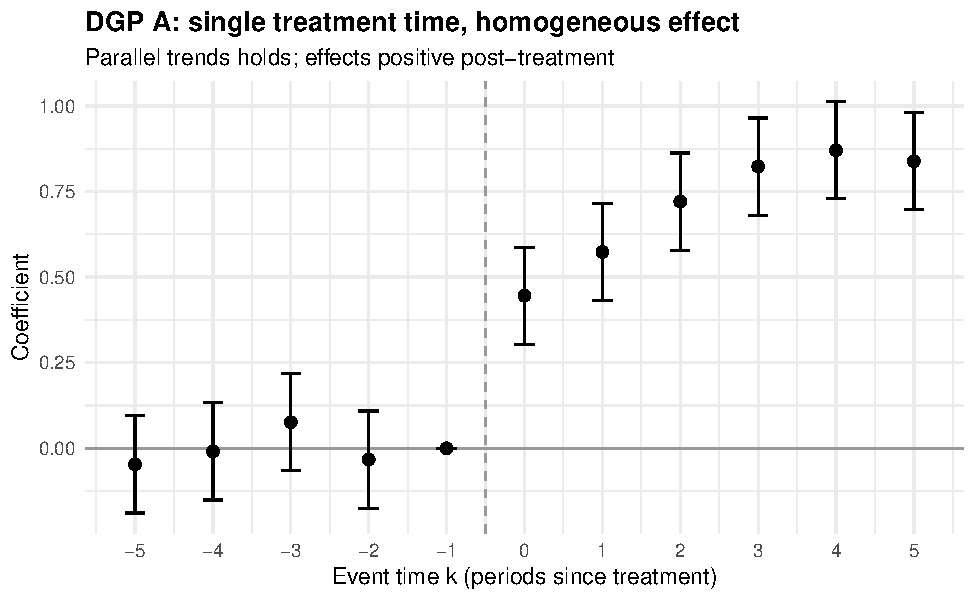
\includegraphics[width=0.68\linewidth]{event_study_clean.pdf}
\end{center}
\end{frame}


\begin{frame}{Event-study design: staggered adoption}
\scriptsize
\textbf{Setup.} DGP B: three cohorts adopted at different times; effect heterogeneous across cohorts. \textit{Parallel trends still holds.} Effects still positive.
\textbf{Same TWFE event-study regression} as before.
\begin{center}
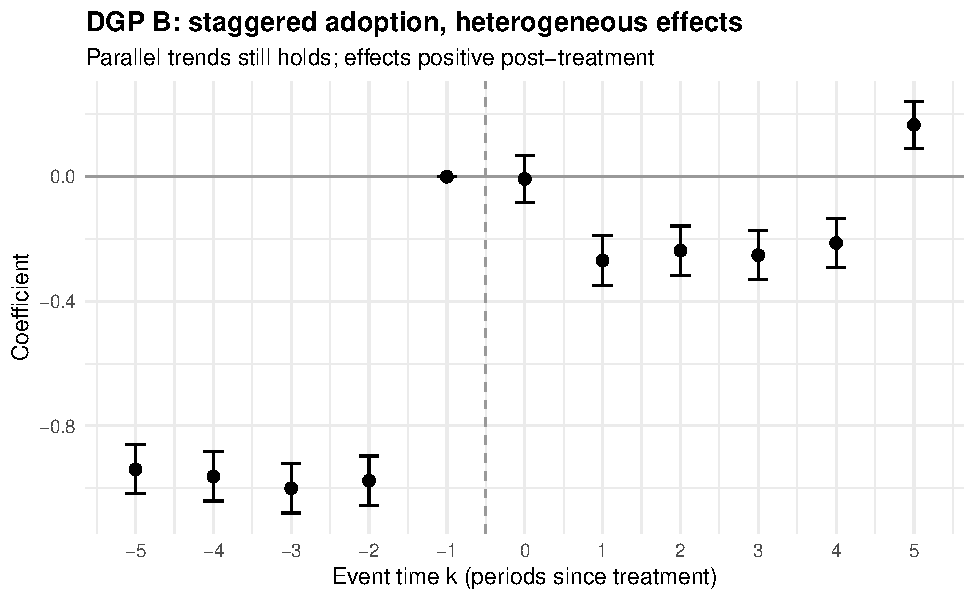
\includegraphics[width=0.62\linewidth]{event_study_contaminated.pdf}
\end{center}
\vspace{-.7em}
\begin{itemize}
\footnotesize
\item Leads appear strongly non-zero---a \textit{false} PT alarm (PT actually holds).
\item Lags flip sign, even though every true cohort-time effect is positive.
\item Pathology is entirely from the estimator, not the DGP.
\item Modern methods (SA, CS, BJS / \texttt{fect}) give event-study plots without it.
\end{itemize}
\end{frame}


\begin{frame}{But remember two things:}
\onslide<1-> Parallel trends is a strong assumption
\small
\begin{itemize}
\item If time-varying influences might lead to treatment and changes in ``growth'', i.e. $Y_t(0)-Y_{t-1}(0)$, then parallel trends is violated. 
\medskip
\item Modern DID methods don't touch this. 
\medskip
\item Parallel trends (in the relevant period) is never testable. Don't be fooled by pre-trend tests. \medskip
\end{itemize} 
\bigskip
\end{frame}

%\begin{frame}[c]\frametitle{How do Elections Affect Government Perfomance?}
%Sances (2013): 
%\begin{itemize}
%  \item Uses original dataset of 920 towns in New York state, over a period where about 400 towns changed their method of choosing property tax officials.
%  \item Plausibly exogenous changes: in 1970, state passes law requiring towns to switch to appointed \textit{unless} they proactively pass a local law via referendum. 
%  \item Clear measure of performance --- how much is the ofifical over or under valuing property?
%\end{itemize}
%
%\end{frame}
%
%\begin{frame}[c]\frametitle{Sances (2013)}
%    \begin{figure}[c]
%      \begin{center}
%        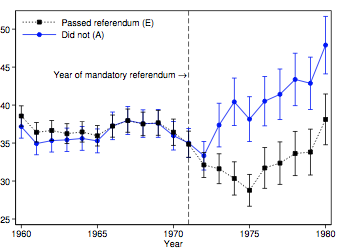
\includegraphics[scale = .8]{sances_1.png}
%      \end{center}
%    \end{figure}
%
%\end{frame}
%
%\begin{frame}[c]\frametitle{Sances (2013)}
%    \begin{figure}[c]
%      \begin{center}
%        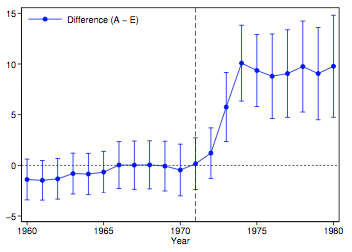
\includegraphics[scale = .8]{sances_2.png}
%      \end{center}
%    \end{figure}
%\end{frame}


\end{document}